\chapter{CO\textsubscript{2} monitoring platform} \label{chap7}
\renewcommand{\headrulewidth}{0pt}
\lhead[\thepage]{\leftmark}
\rhead[\leftmark]{\thepage}
\cfoot[]{}

\section{Introduction}

The widely acknowledged importance of climate change across various aspects \citep{primack2009impact, watanabe2009general, ogawa2013ecological, shibuya2016effect} is driving an accelerated momentum toward achieving Carbon Neutrality (CN) in local Japanese governments \citep{nakazawa2023net}. In both major corporations and small businesses, there is a rising demand for the measurement of greenhouse gas (GHG) emissions \citep{kauffmann2012corporate}. Companies are mandated to visualize their CO\textsubscript{2} emissions and implement measures to reduce them. As of September 2023, 991 local governments, including Tokyo, Kyoto, and Yokohama, have demonstrated increased enthusiasm for this initiative by declaring their commitment to achieving net-zero carbon emissions by 2050 \citep{zerocarboncities}. However, to specifically implement mitigation and adaptation measures, it is necessary to perform comprehensive risk analysis and calculate detailed emissions for each sector. Furthermore, it is required to visualize this information in an easy-to-understand manner in time and space, and to explain and disclose it to various stakeholders. On the other hand, in recent years, local governments have been accelerating the integration of map information that had previously been prepared separately for each department, such as taxation, urban planning, and the environment. Integrated geographic information systems (GIS) enable cross-sectional analysis of various elements, have become one of the cornerstones of administrative digital transformation (DX), and have been introduced in 60\% of all 1,741 municipalities \citep{nikkei}.\par

By using WebGIS functions, local CN-related policy makers can monitor energy consumption and CO\textsubscript{2} emissions by sector such as industry, electricity, transportation, buildings and housing. By integrating it into the Geo-portal site, it will be possible to better understand the actual situation and make appropriate plans to introduce renewable energy and reduce emissions. However, for example, although national energy consumption and power generation can be determined from the regional energy supply and demand database \citep{Toshihiko} and the electric power database \citep{kitamoto, nlftp}, the visualization systems for these databases have been developed separately, therefore it is difficult for policy makers to analyze comprehensibly and make integrated planning.\par

In this chapter, we presented a case study illustrating the development of a comprehensive tool for developing a "Supporting and Visualizing Carbon Neutrality (CN) Roadmap". This tool serves as a Digital Earth application designed to aid Japanese local governments in their pursuit of CN goals. To achieve CN, it is necessary to create cost-effective roadmaps (scenarios) based on the characteristics of each region and local government. Drafting such scenarios requires a comprehensive understanding of energy use and CO\textsubscript{2} emission patterns in each sector. The Project Drawdown \citep{brennan2020project}, a prominent initiative in this realm, represents a collaborative effort among multidisciplinary scientists, researchers, and practitioners. Its primary objective is to identify and advocate for the most impactful solutions to mitigate and potentially reverse global warming. A research group composed of researchers and policymakers has formulated and recommended various solutions for reducing greenhouse gas emissions. Despite these proposals, none of the tools have been fully integrated into the GIS platform. The integration of greenhouse gas (GHG) monitoring and zero carbon roadmap simulation into GIS platforms is currently under exploration within the Digital Earth platform \citep{fukui2021digital}. Consequently, we are engaged in research and development efforts aimed at creating a Digital Earth-based platform. This platform is designed to furnish policymakers with comprehensive roadmaps, progress tracking toward goals, and other pertinent information, all within a unified GIS platform (Figure \ref{fig:chap7_fig1}). \par

\section{Method}
Figure \ref{fig:chap7_fig1} depicts the components of the GIS platform established in this study and the core technologies utilized in its development. Initially, the process involves collecting, preprocessing, and archiving CO\textsubscript{2} emissions and related data from various sources. This data is then made available to end-users for visualization and other purposes through the development of Application Programming Interfaces (APIs). The API is designed to encompass two main functionalities: the CO\textsubscript{2} Emissions Tracker and Zero Carbon Modeling (also referred to as Drawdown). In the CO\textsubscript{2} Emissions section, users can analyze trends and patterns in CO\textsubscript{2} emissions. In the Zero Carbon Modeling (Drawdown) section, roadmaps are presented for 1,741 municipalities, each delineating effective reduction strategies for achieving carbon neutrality by 2050.\par
\begin{figure}
  \centering
  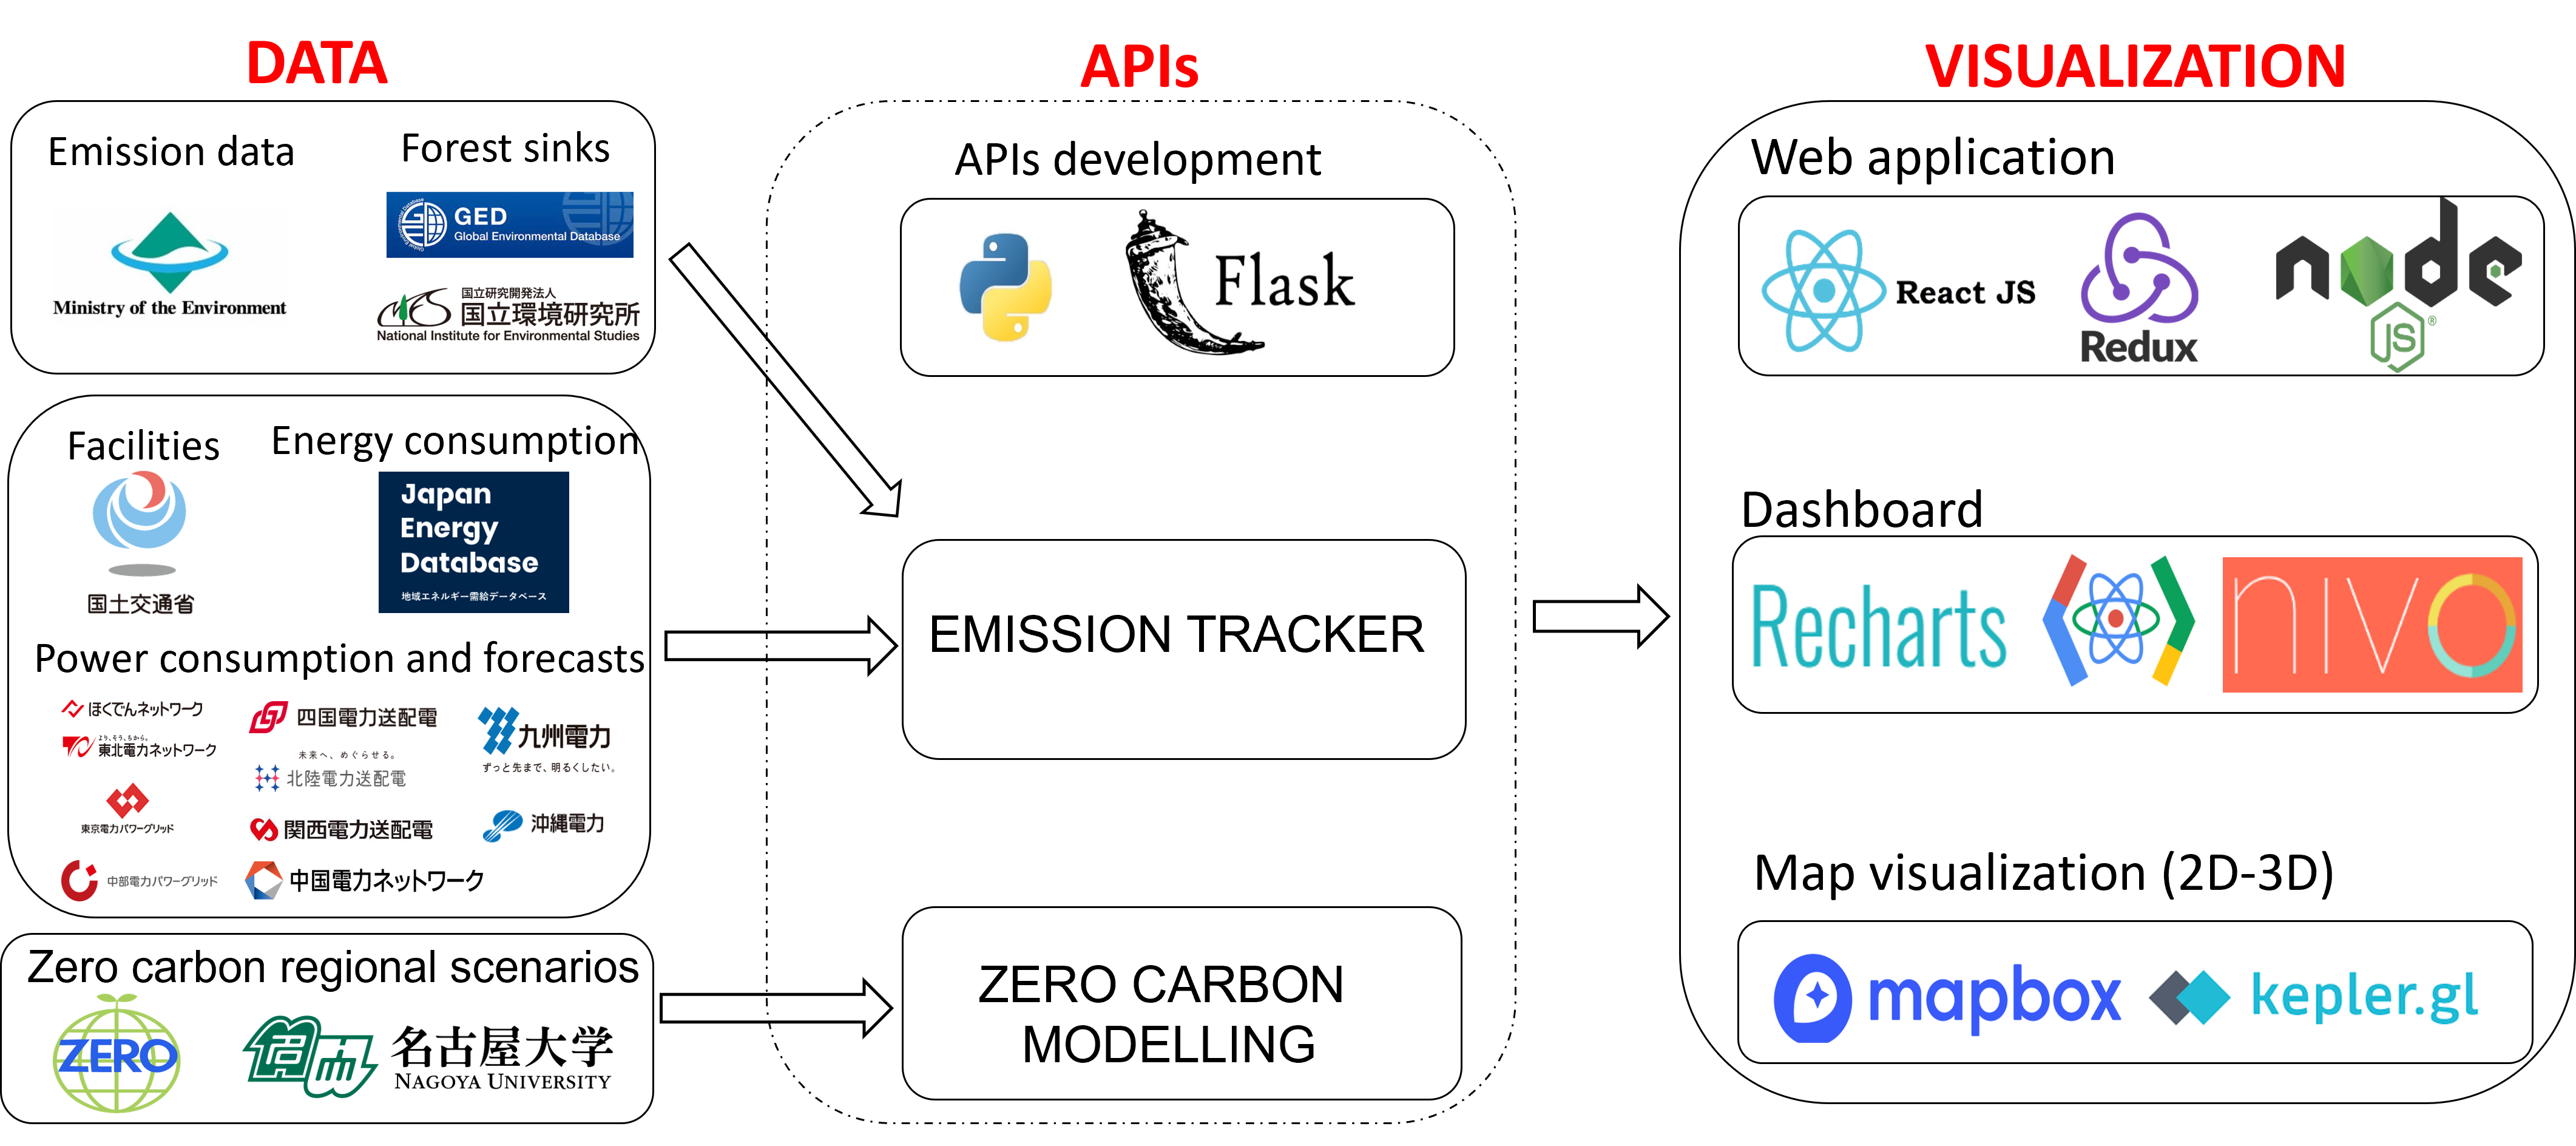
\includegraphics[width=\textwidth]{figs/chap7/platform_architecture.png}
  \caption[Platform architecture]{Platform Architecture and the technology used to develop the GIS platform}
  \label{fig:chap7_fig1}
\end{figure}

\subsection{Data collection}
Table \ref{tab:chap7_tab1} compiles information on datasets integrated into the GIS platform, along with their respective data sources. All data utilized underwent collection or preprocessing to maintain original resolution and municipality granularity. \par

\begin{table}[!ht]
    \centering
    \caption{The dataset used for the GIS platform development}
    \begin{adjustbox}{width=\textwidth}
        \begin{tabular}{l l}
        \hline
            Dataset & Data source \\ \hline
            CO\textsubscript{2} emissions by sector & \citep{env2022} \\ \hline
            Energy consumption statistics & \citep{Toshihiko} \\ \hline
            Power generation facility & \citep{nlftp} \\ \hline
            \multirow{10}{*}{Power consumption and forecasts} & \citep{hokkaido} \\
            ~ & \citep{tohoku} \\
            ~ & \citep{Tokyo} \\
            ~ & \citep{Chubu} \\
            ~ & \citep{Hokuriku} \\
            ~ & \citep{Kansai} \\
            ~ & \citep{Chugoku} \\
            ~ & \citep{Shikoku} \\
            ~ & \citep{Kyushu} \\
            ~ & \citep{Okinawa} \\ \hline
            Gross Primary Production & \multirow{3}{*}{\citep{ito2019disequilibrium}} \\
            Net Ecosystem Production & ~ \\
            Ecosystem respiration & ~ \\ \hline
            Zero carbon regional scenario & \citep{zerocarbon} \\
            \hline
        \end{tabular}
    \end{adjustbox}
    \label{tab:chap7_tab1}
\end{table}

Initially, for monitoring current greenhouse gas emissions and energy-related issues, we employed diverse data sources. Specifically, we utilized CO\textsubscript{2} emission estimates by sectors from \citep{env2022} to visualize the overall emission landscape. Additionally, we delved into industrial emissions details, using data from the Ministry of the Environment spanning 2009 to 2017. To depict forest sink capabilities, we incorporated three terrestrial carbon flux variables—gross primary production, net ecosystem production, and ecosystem respiration—from \citep{ito2019disequilibrium}. For presenting energy-related information, energy consumption data from \citep{Toshihiko} showcased the contrast between 2013 and 2019. The distribution of power plants across the country was illustrated using data from \citep{nlftp}. To offer near-real-time power consumption, we utilized data from 10 electric power companies, as outlined in Table \ref{tab:chap7_tab1}, showcasing power consumption and forecasts.\par

Subsequently, we integrated data from the Zero Carbon Region Scenario Analysis Tool \citep{zerocarbon}, specifically designed to assist municipal staff in identifying and achieving CO\textsubscript{2} reduction targets for 2030, 2040, and 2050 to attain net-zero carbon by 2050. This information was utilized to generate corresponding maps and charts for visualization.\par

\subsection{API development}
In the development of the API for handling this data, we employed Flask \citep{grinberg2018flask}, a lightweight web framework coded in Python, and conformed to the JSON API specification for data formatting. The API within this system is responsible for rendering dashboards related to Emission Tracker and Zero Emission Modeling (Drawdown). JSON functions as the predominant data format for the API, with all responses aligning with the specifications outlined in Table \ref{tab:chap7_tab2}. The APIs are deployed on the cloud-based platform Heroku, and the interfaces are depicted in Figure \ref{fig:chap7_fig_api}. \par

\begin{table}[!ht]
  \centering
  \caption{APIs specifications}
  \begin{adjustbox}{width=\textwidth}
      \begin{tabular}{lll}
        \hline
        End point & Parameters & Description \\ \hline
        \multicolumn{3}{l}{Base URL: https://emissionjp.herokuapp.com/ems\_tracker/} \\ \hline
        GET /overall\_ems/country  & year: year of the emission data  & Emissions at national level \\ \hline
        \multirow{2}{*}{GET /overall\_ems/municipality}  & adm\_code: municipality code  & Emissions at municipality level in a specific year \\ 
        ~ & year: year of the emission data  & ~ \\ \hline
        GET /overall\_ems/municipality\_ts  & adm\_code: municipality code  & Time-series emissions at municipality level.  \\ \hline
        GET /overall\_ems/sector  & sector\_type: sector type & Emissions categorized by sectors.  \\ \hline
        GET /ee\_stats/5mins  & None & Near real time power usage, forecast \\ \hline
        GET /ee\_stats/energy\_consumption  & adm\_code: municipality code  & Energy consumption at municipality level.  \\ \hline
        GET /forest\_sink/municipality  & adm\_code: municipality code  & Forest variable at municipality level.  \\ \hline
        \multirow{2}{*}{GET /industry/annual\_ems}  & adm\_code: municipality code & Industrial emission at municipality level \\ 
        ~ & year: year of the emission data & ~ \\ \hline
        \multicolumn{3}{l}{Base URL: https://emissionjp.herokuapp.com/zero\_ems/} \\ \hline
        GET /zero\_ems/municipality & adm\_code: municipality code & Roadmap to reduce GHG at municipality level \\ \hline
    \end{tabular}
  \end{adjustbox}
  \label{tab:chap7_tab2}
\end{table}

We present examples of two API responses, achieved through the execution of a GET request directed to two distinct endpoints: /overall\_ems/municipality for generating a map visualization and /overall\_ems/municipality\_ts for generating a line chart visualization specific to a municipality. This demonstration offers a clear and practical example of the API's functionality. Users can initiate these requests without the need for authentication.  \par

\begin{lstlisting}[language=json,firstnumber=1, basicstyle=\small, caption={A response from GET /overall\_ems/municipality },captionpos=t]
  {
    "features": [
      {
        "geometry": {
          "coordinates": [[...]],
          "type": "Polygon"
        },
        "id": "26",
        "properties": {
          "adm_code": 23100,
          "agriculture": 30,
          "building": 3435,
          "business": 5034,
          "city": "Nagoya Shi",
          "construction_mining": 235,
          "consumer_total": 8469,
          "freight_car": 1222,
          "industry_total": 3900,
          "manufacture": 3635,
          "passenger_car": 2134,
          "pref": "Aichi Ken",
          "pref_code": 23,
          "railway": 126,
          "ship": 46,
          "total": 16017,
          "transportation_total": 3528,
          "waste": 121
        },
        "type": "Feature"
      }
    ],
    "type": "FeatureCollection"
  }
\end{lstlisting}
\begin{lstlisting}[language=json,firstnumber=1, basicstyle=\small, caption={A response from GET /overall\_ems/municipality\_ts},captionpos=t]
  {
  "result": [
    {
      "agriculture": 39,
      "building": 2473,
      "business": 3032,
      "construction_mining": 311,
      "freight_car": 1478,
      "manufacture": 6910,
      "passenger_car": 1840,
      "railway": 133,
      "ship": 36,
      "waste": 144,
      "year": 1990
    },
    ...
    {
      "agriculture": 30,
      "building": 3435,
      "business": 5034,
      "construction_mining": 235,
      "freight_car": 1222,
      "manufacture": 3635,
      "passenger_car": 2134,
      "railway": 126,
      "ship": 46,
      "waste": 121,
      "year": 2005
    },
  ]
}
\end{lstlisting}

\begin{figure}[tbh!]
  \centering
  \begin{subfigure}{.5\textwidth}
      \centering
      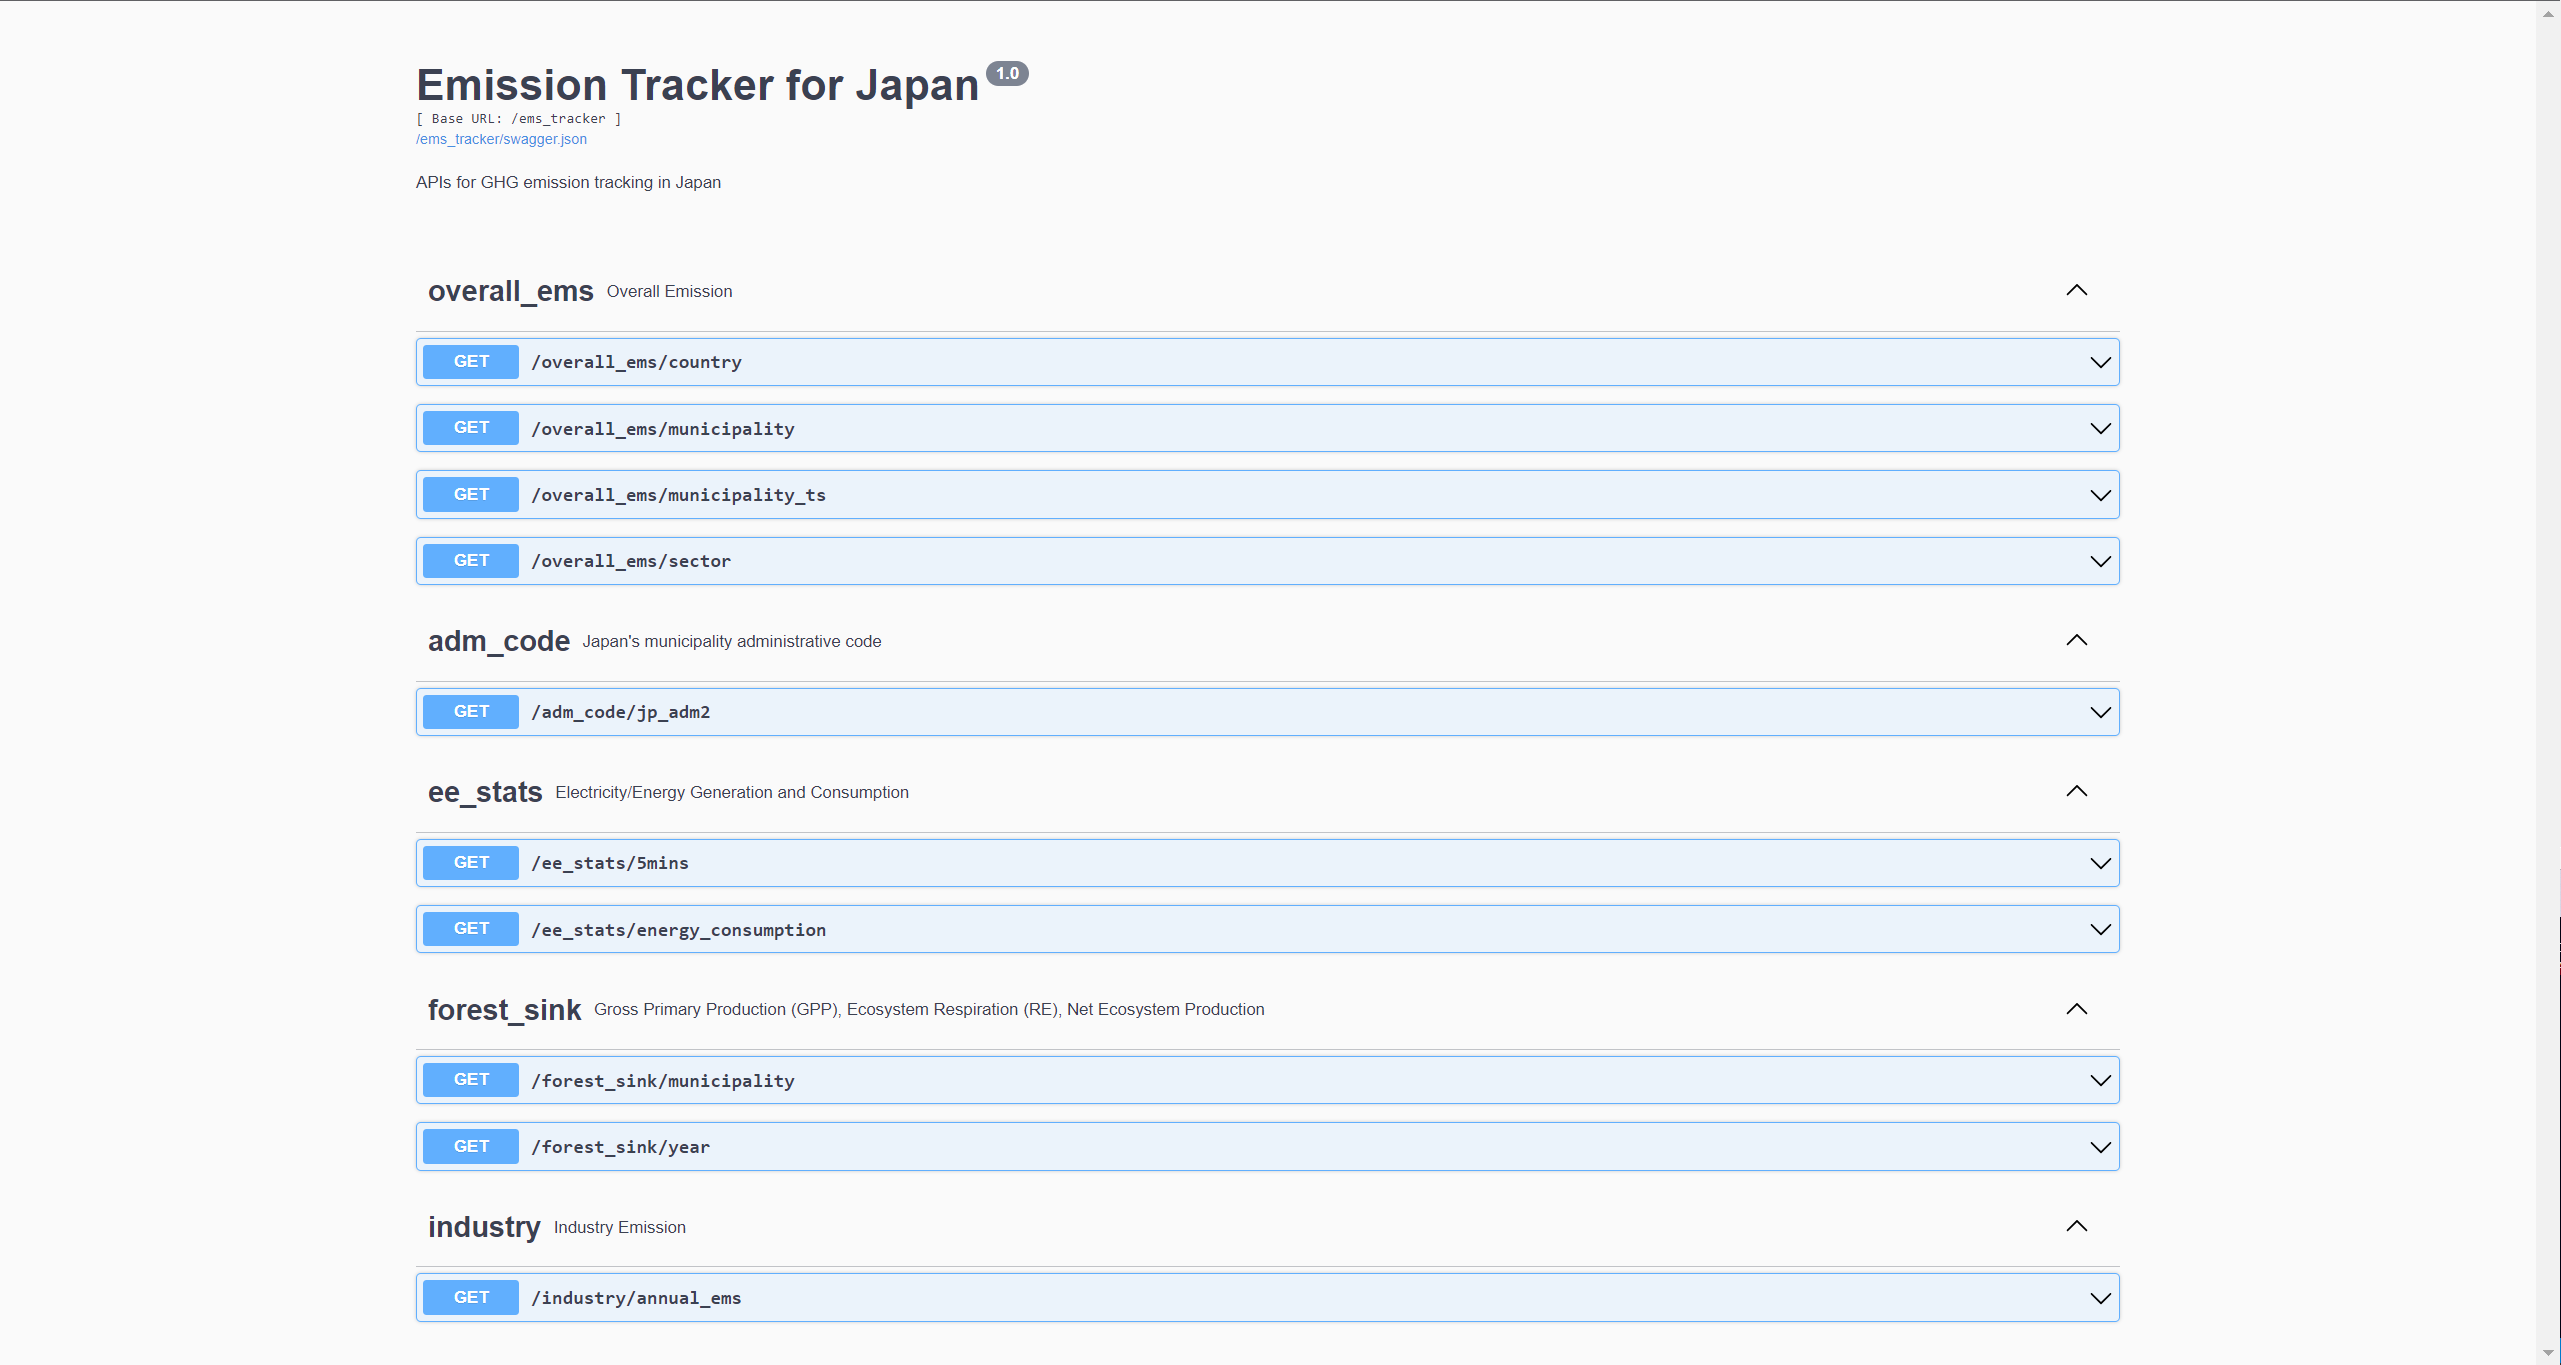
\includegraphics[width=.9\textwidth]{figs/chap7/api1.png}
      \caption{Emission Tracker APIs}
  \end{subfigure}%
  \begin{subfigure}{.5\textwidth}
      \centering
      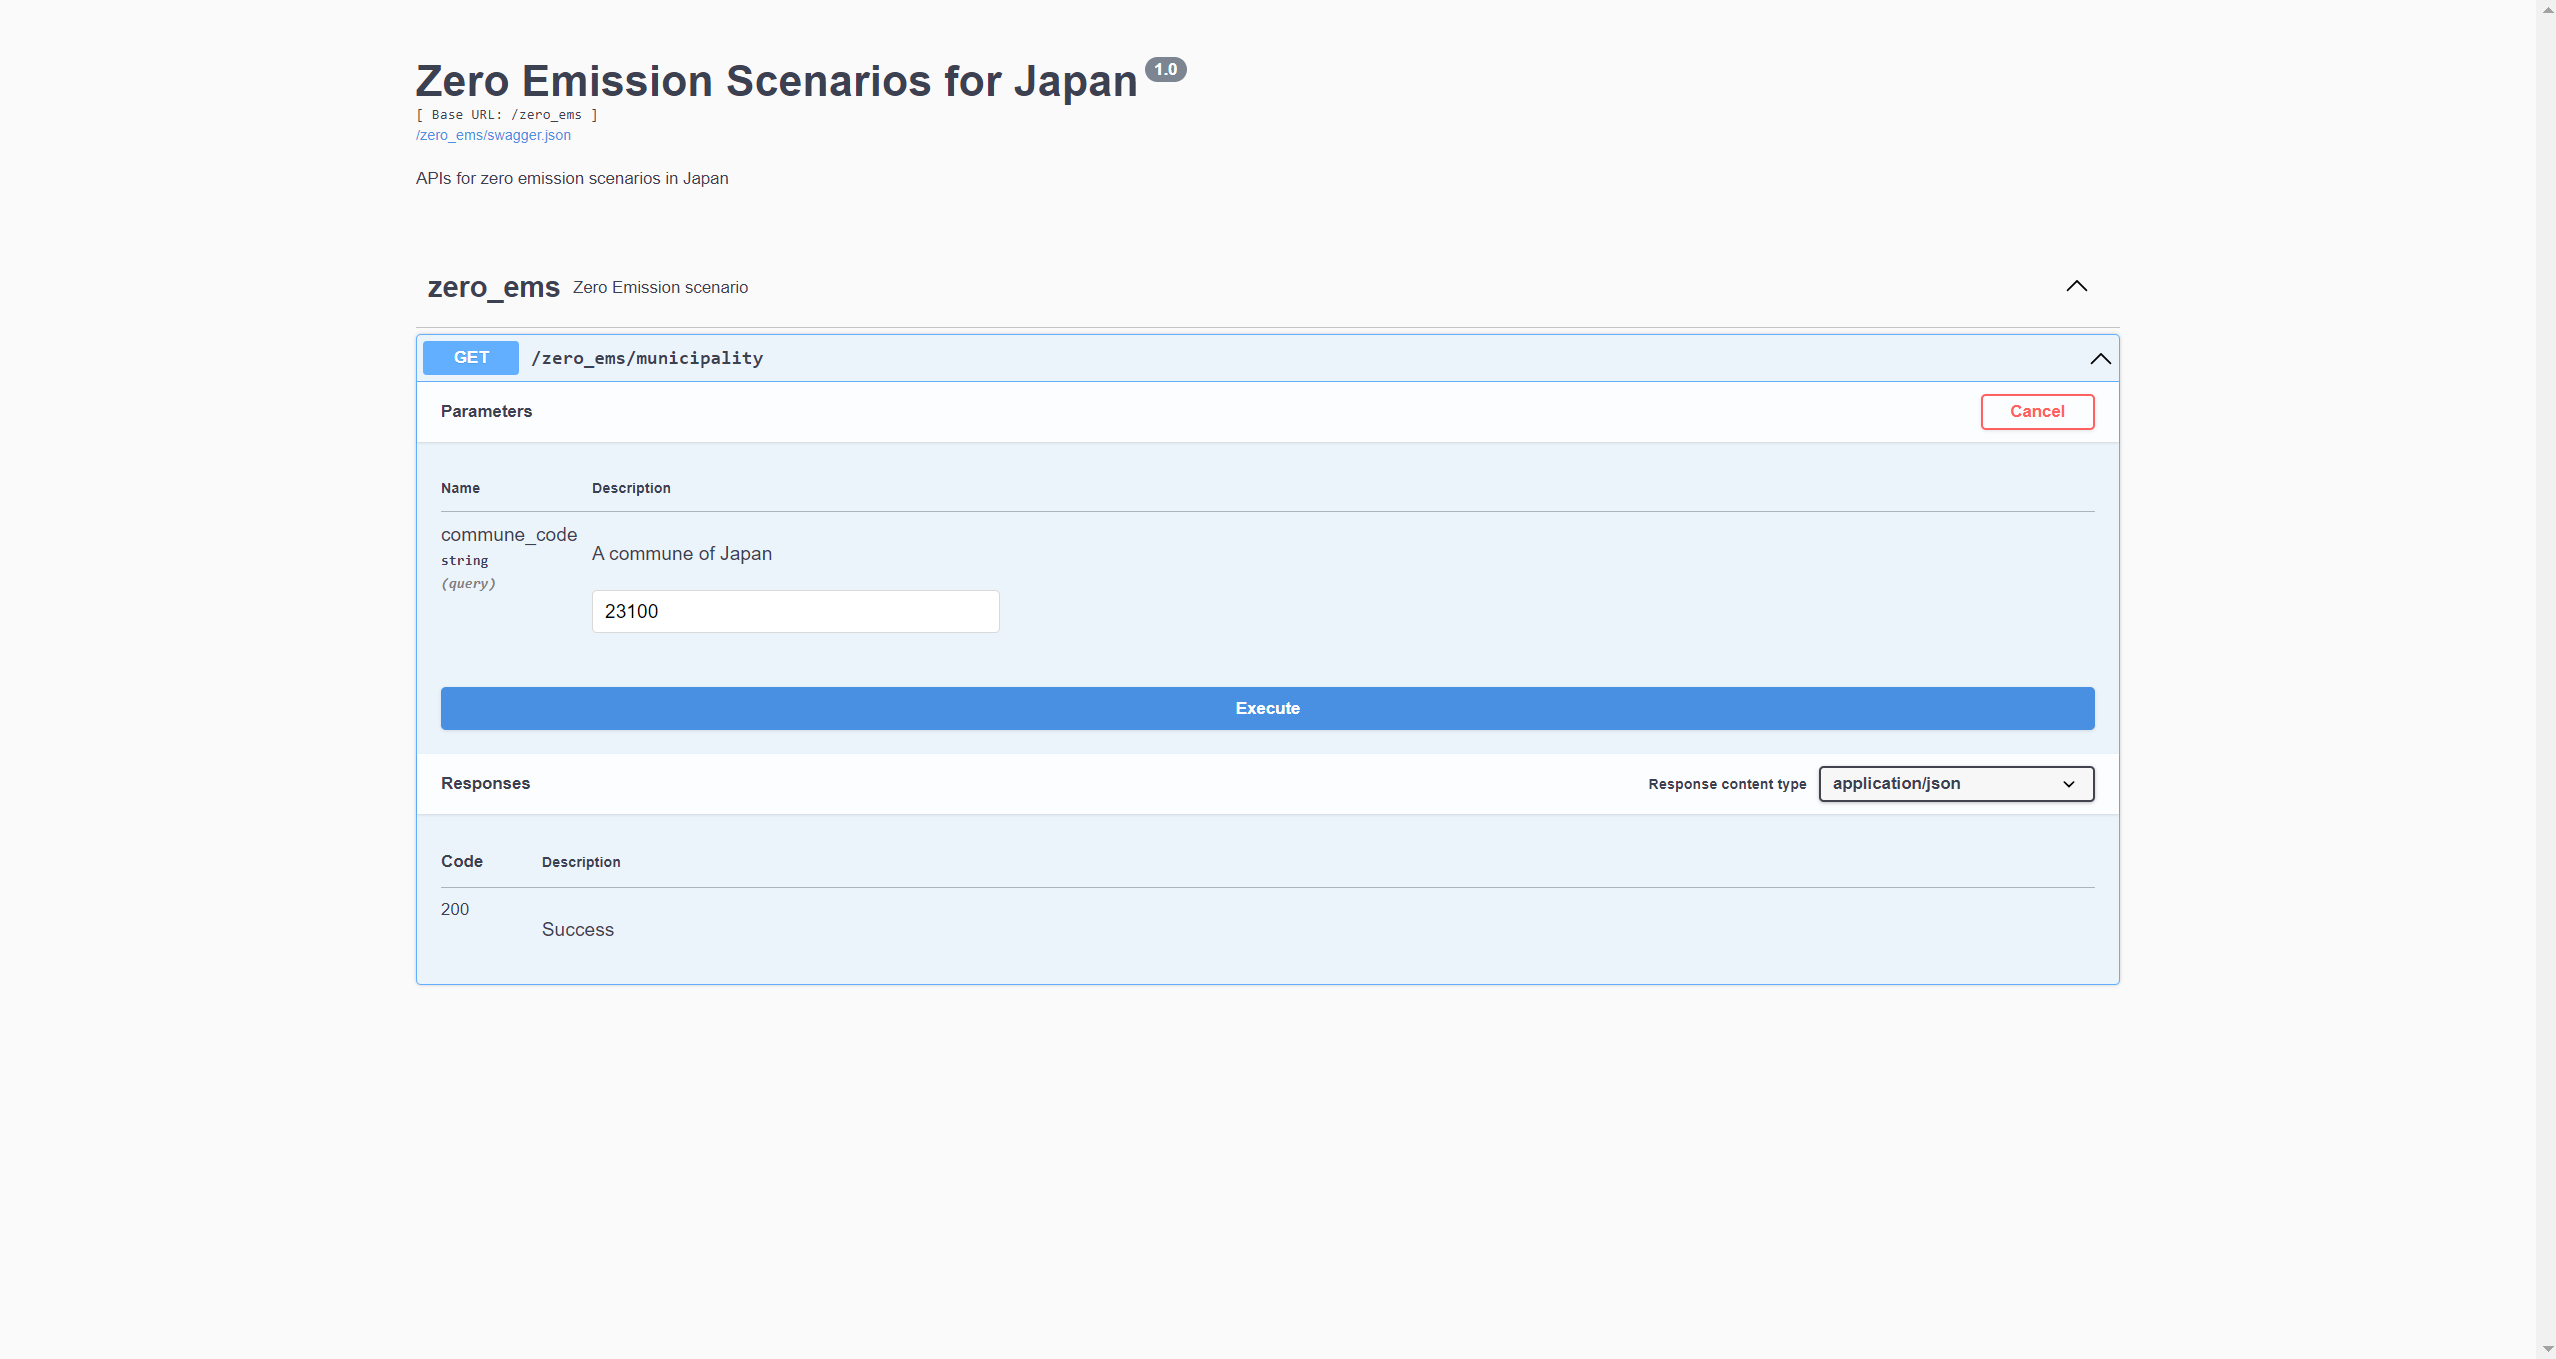
\includegraphics[width=.9\textwidth]{figs/chap7/api2.png}
      \caption{Zero Emission API}
  \end{subfigure}
  \caption{APIs interfaces Emission Tracker APIs (a) Zero Emission APIs (b)}
  \label{fig:chap7_fig_api}
\end{figure}


\subsection{Web application}

The web application comprises two primary functionalities: (1) tracking greenhouse gas (GHG) emissions, referred to as the Emissions Tracker, and (2) modeling scenarios for achieving zero-carbon emissions, known as Drawdown. The objective of the GHG emission tracker is to offer a comprehensive overview of emissions and forest sinks at the municipality level. Additionally, we provide data on energy consumption to enhance end-users' understanding of the current situation. To achieve this, we have organized the GHG emission tracker into five specific tabs: Emission Overview, Forest Sinks, Energy Consumption, Electricity Statistics, and Industrial Emission. In the context of Drawdown modeling, we present simulation results that serve as a roadmap for maximizing emission reduction by 2050. To construct the interactive and informative GIS dashboard, we utilized the following technologies for platform development. \par
\begin{itemize}
  \item Web Application: Node.js, ReactJS, Redux
  \item Interactive Charts: Rechart, React Google Charts, NIVO
  \item Interactive Maps: Mapbox and Kepler.gl
\end{itemize}

\section{Result and discussion}
\subsection{Result}
The summary of usage scenarios for the created GIS platform is presented below. Initially, we delve into the interface of Emission Tracker-related pages (see Figure \ref{fig:chap7_fig_ems_tracker}) and the Drawdown page {see Figure \ref{fig:chap7_fig_drawdown}}. Subsequently, we elaborate on other functionalities of the platform (see Figure \ref{fig:chap7_fig_other_interface}). \par

\begin{figure}[tbh!]
  \centering
  \begin{subfigure}{.5\textwidth}
      \centering
      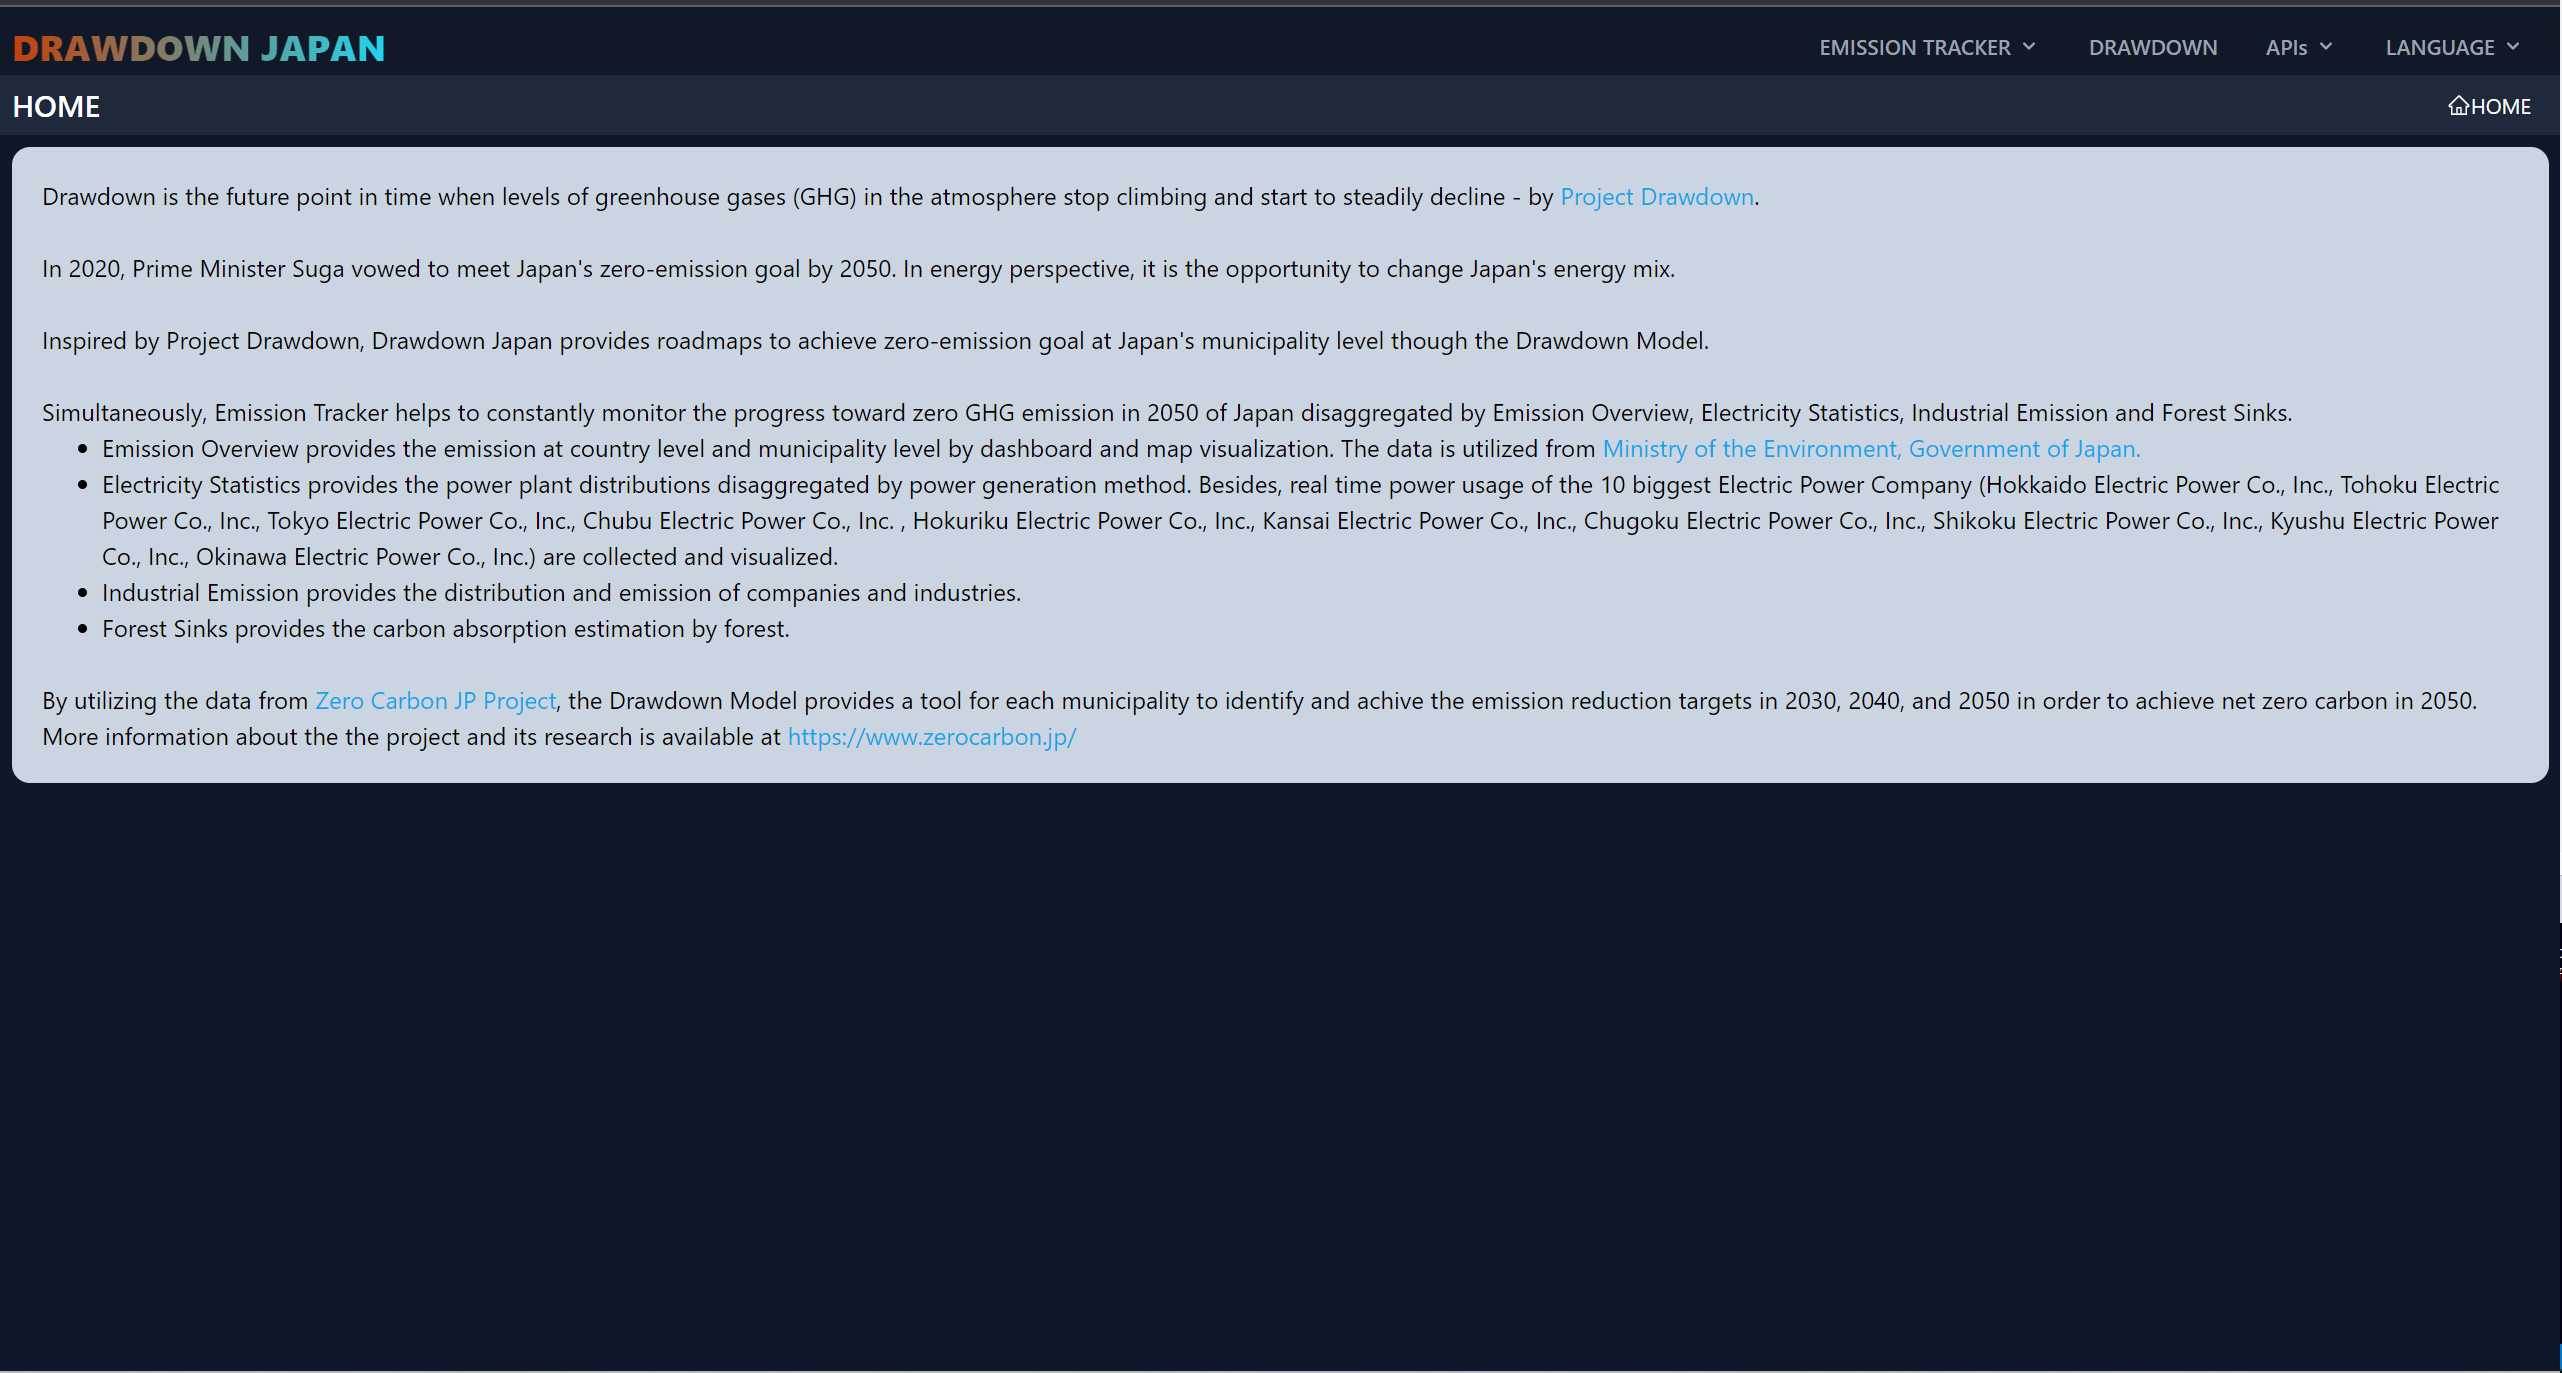
\includegraphics[width=.9\textwidth]{figs/chap7/home.png}
      \caption{Home page}
  \end{subfigure}%
  \begin{subfigure}{.5\textwidth}
      \centering
      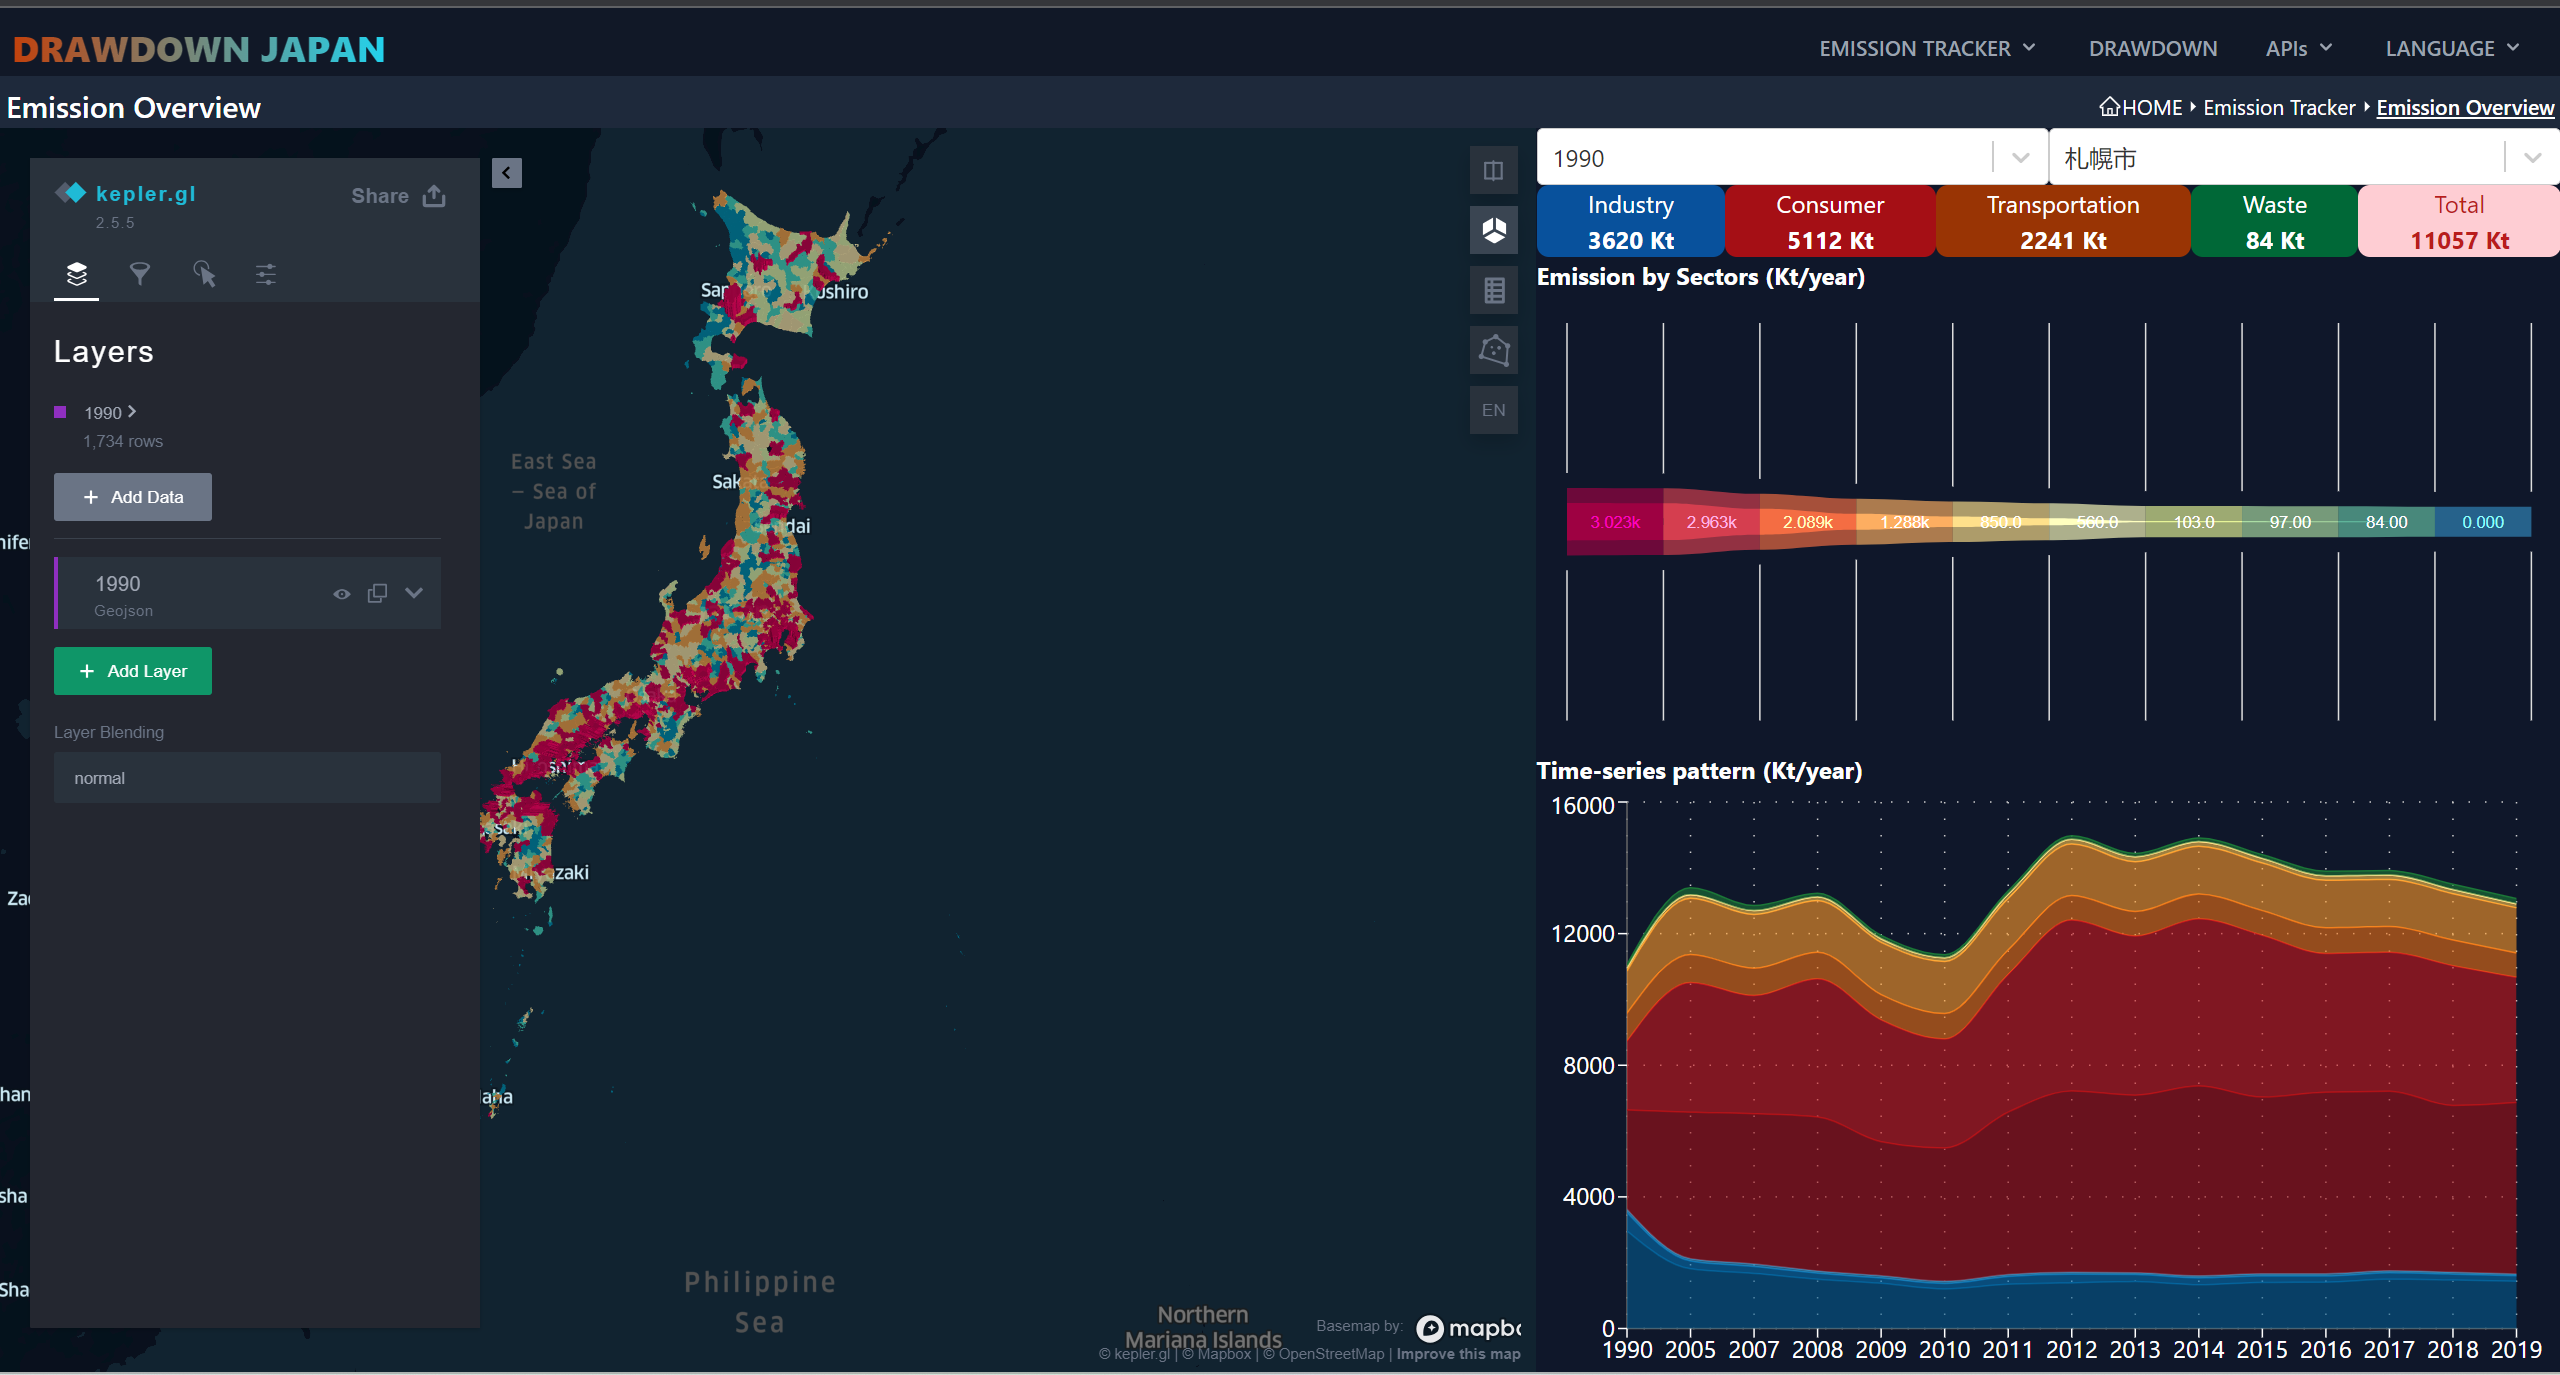
\includegraphics[width=.9\textwidth]{figs/chap7/ems_overview.png}
      \caption{Emission Overview}
      \label{fig:chap7_fig_ems_tracker_a}
  \end{subfigure}

  \begin{subfigure}{.5\textwidth}
      \centering
      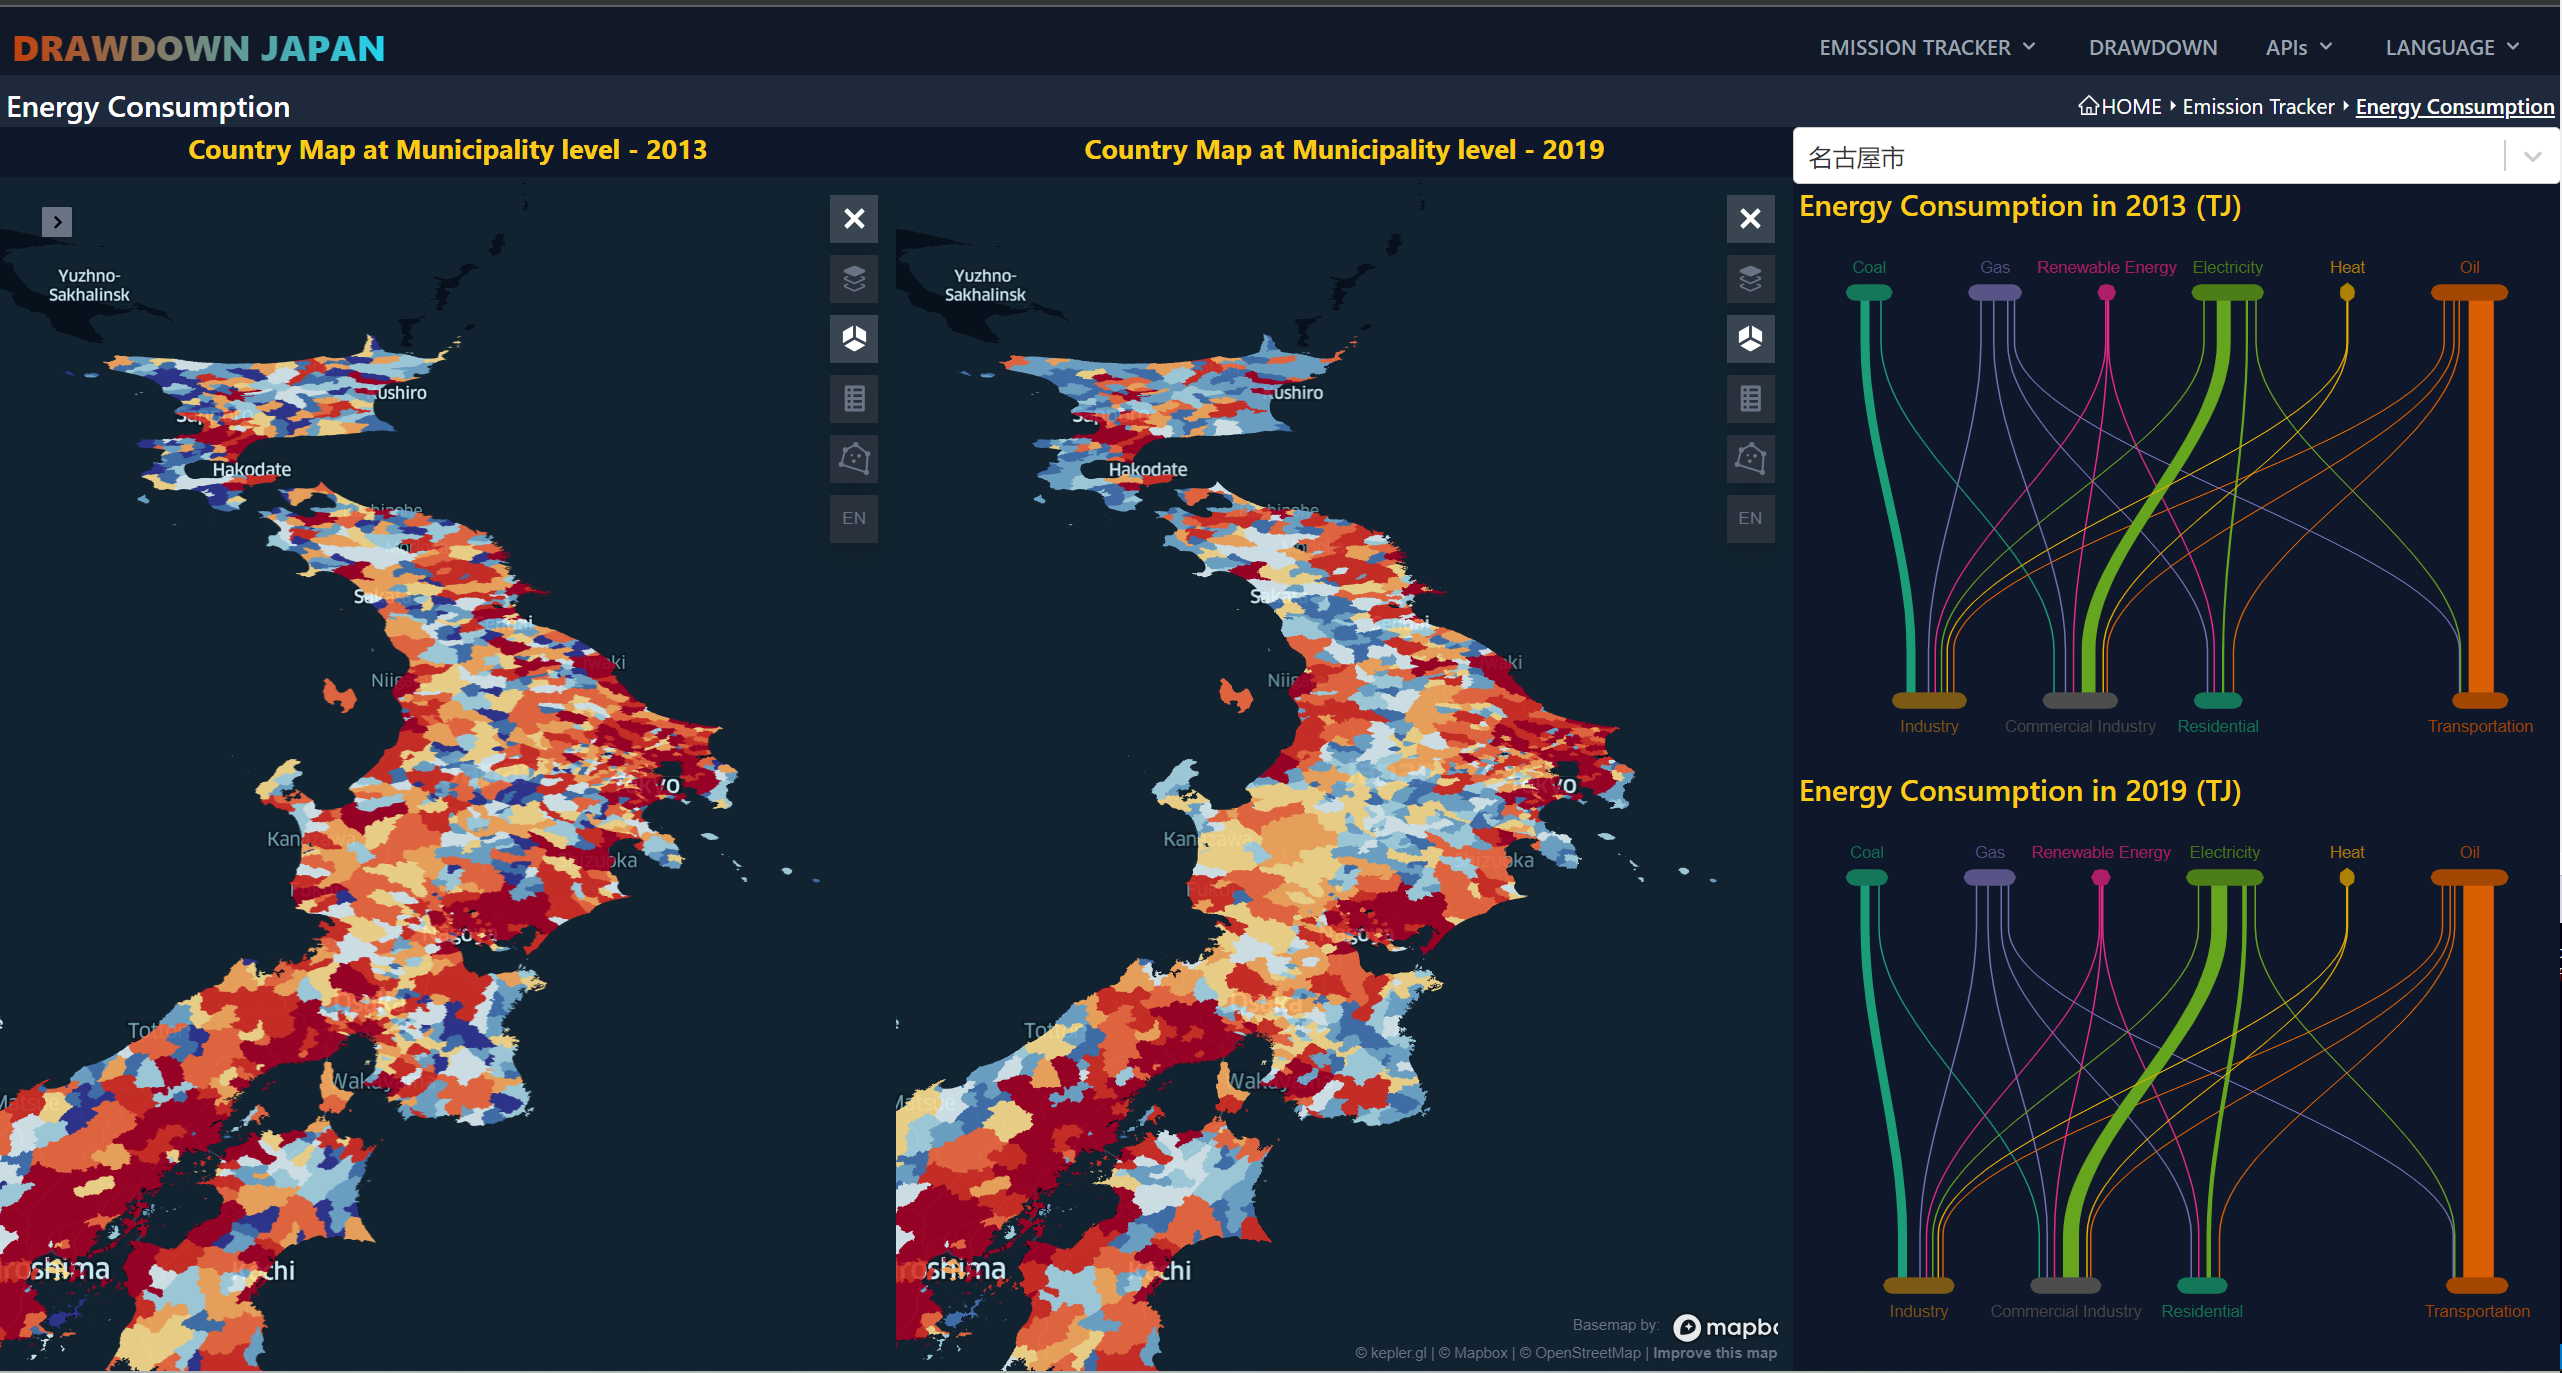
\includegraphics[width=.9\textwidth]{figs/chap7/ems_consumption.png}
      \caption{Energy Consumption}
      \label{fig:chap7_fig_ems_tracker_b}
  \end{subfigure}%
  \begin{subfigure}{.5\textwidth}
      \centering
      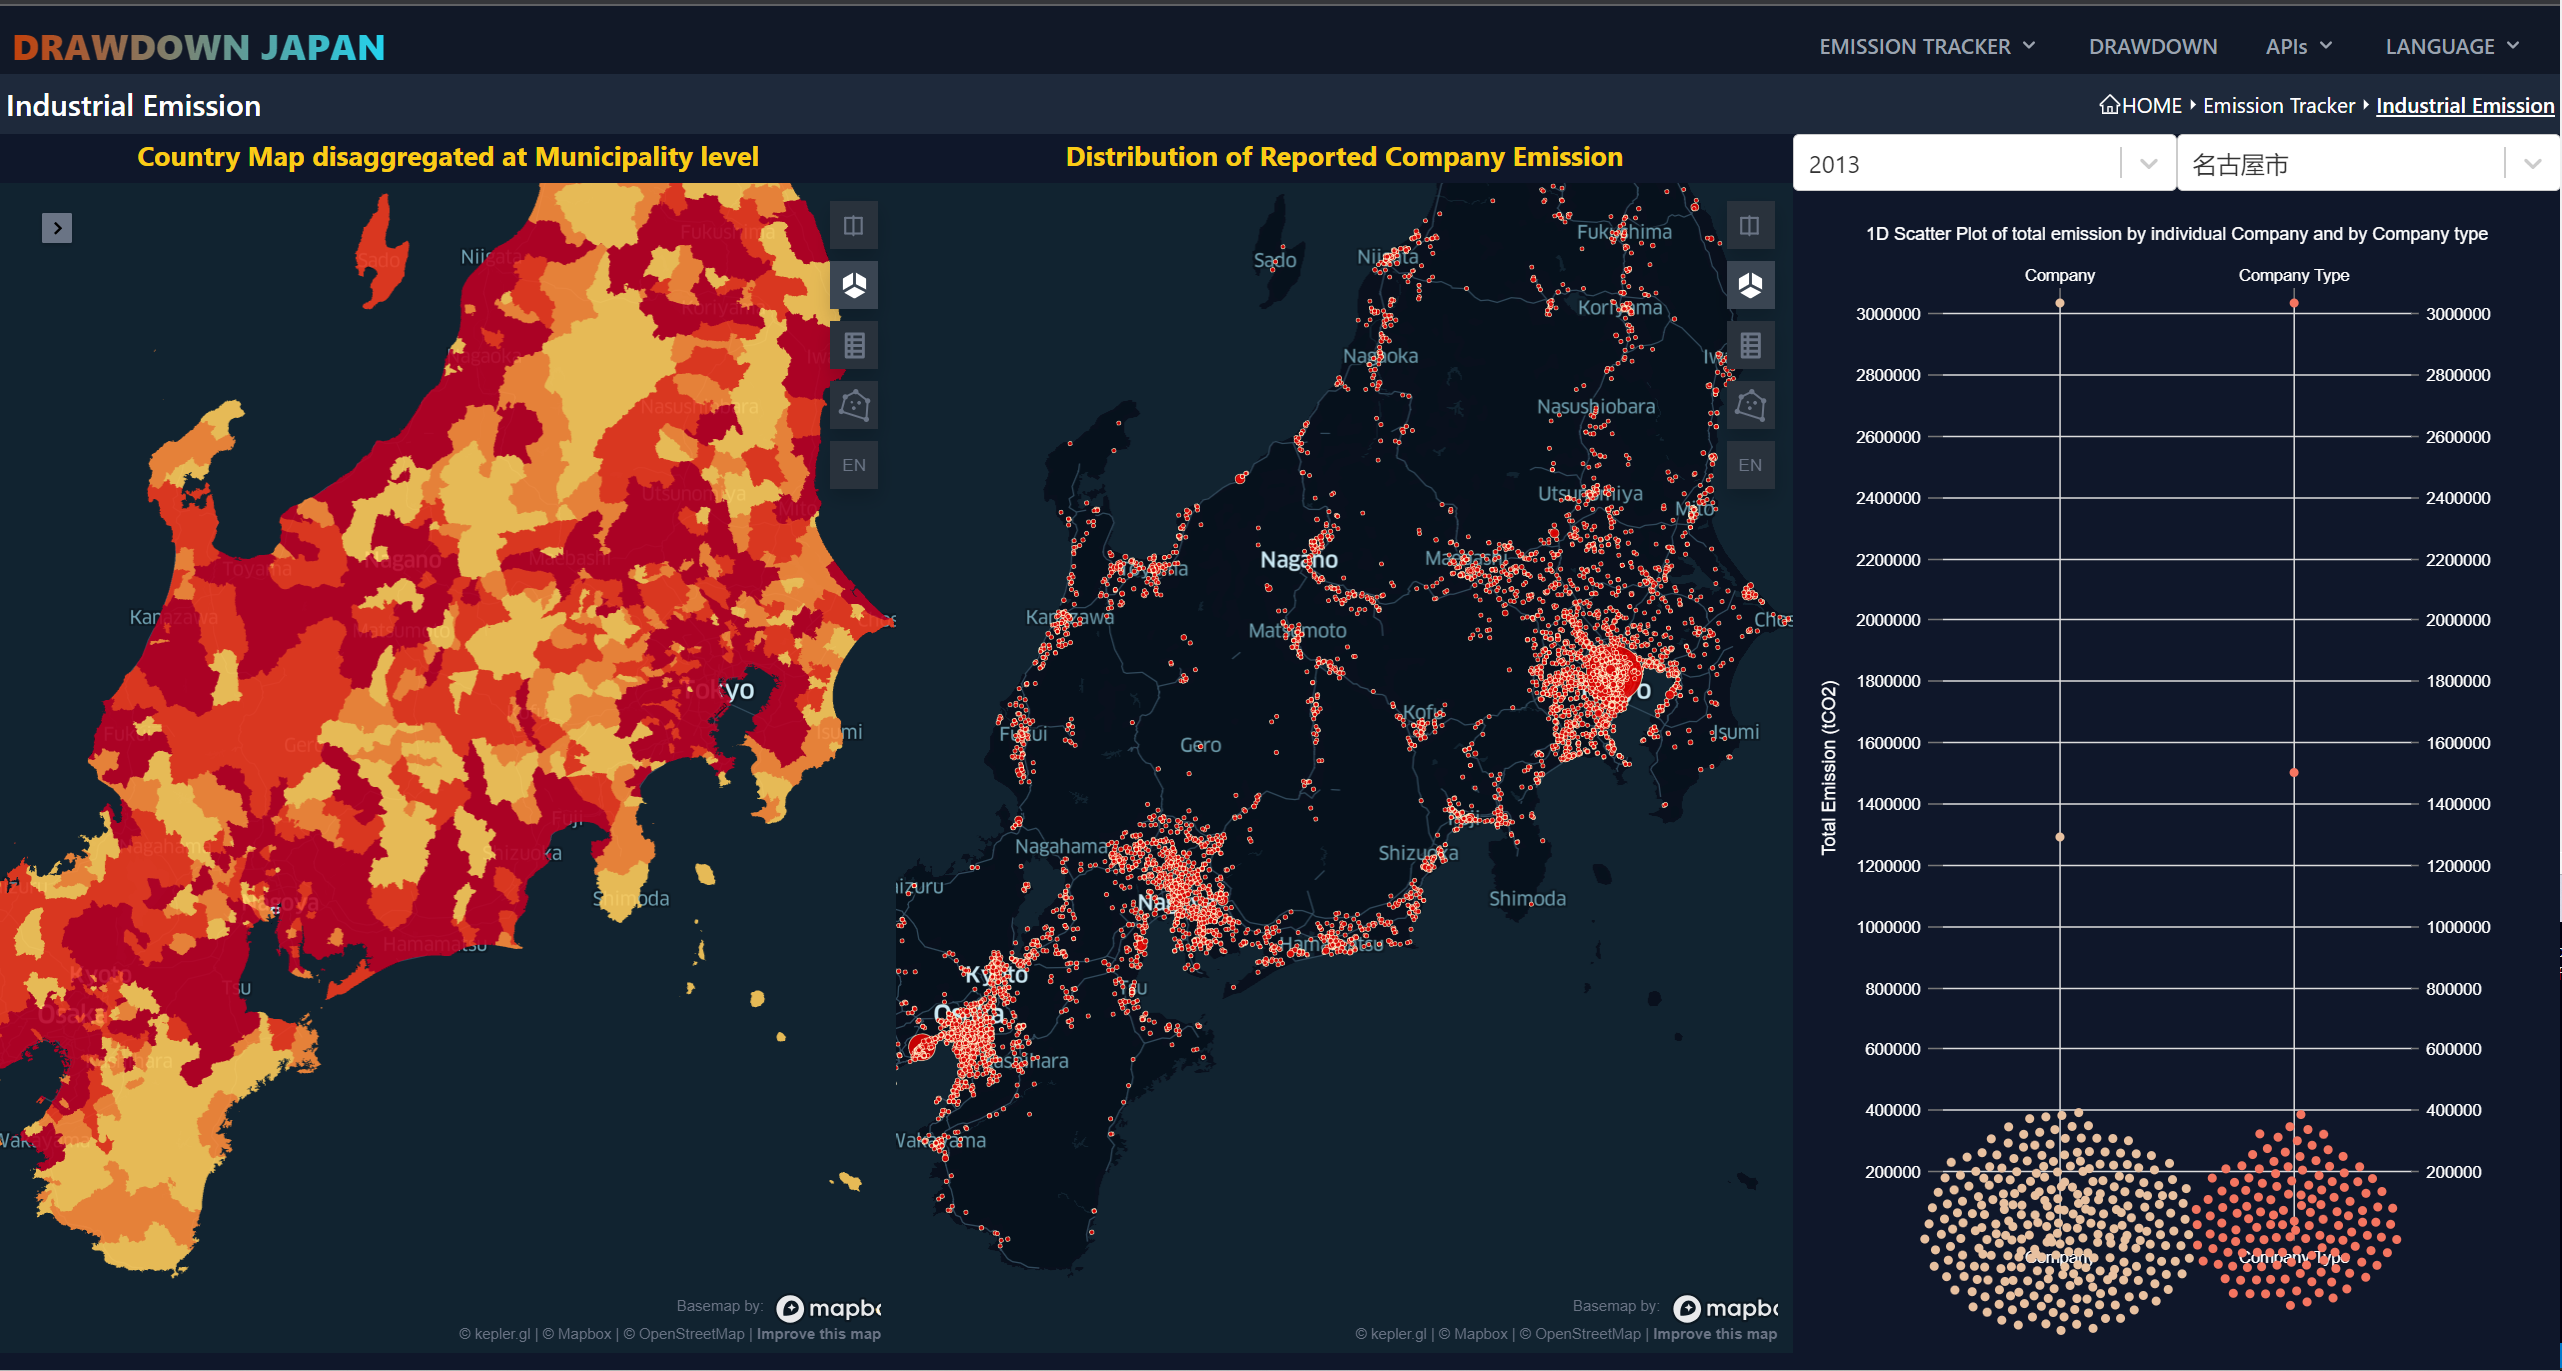
\includegraphics[width=.9\textwidth]{figs/chap7/industrial_ems.png}
      \caption{Industrial Emission}
      \label{fig:chap7_fig_ems_tracker_c}
  \end{subfigure}

  \begin{subfigure}{.5\textwidth}
    \centering
    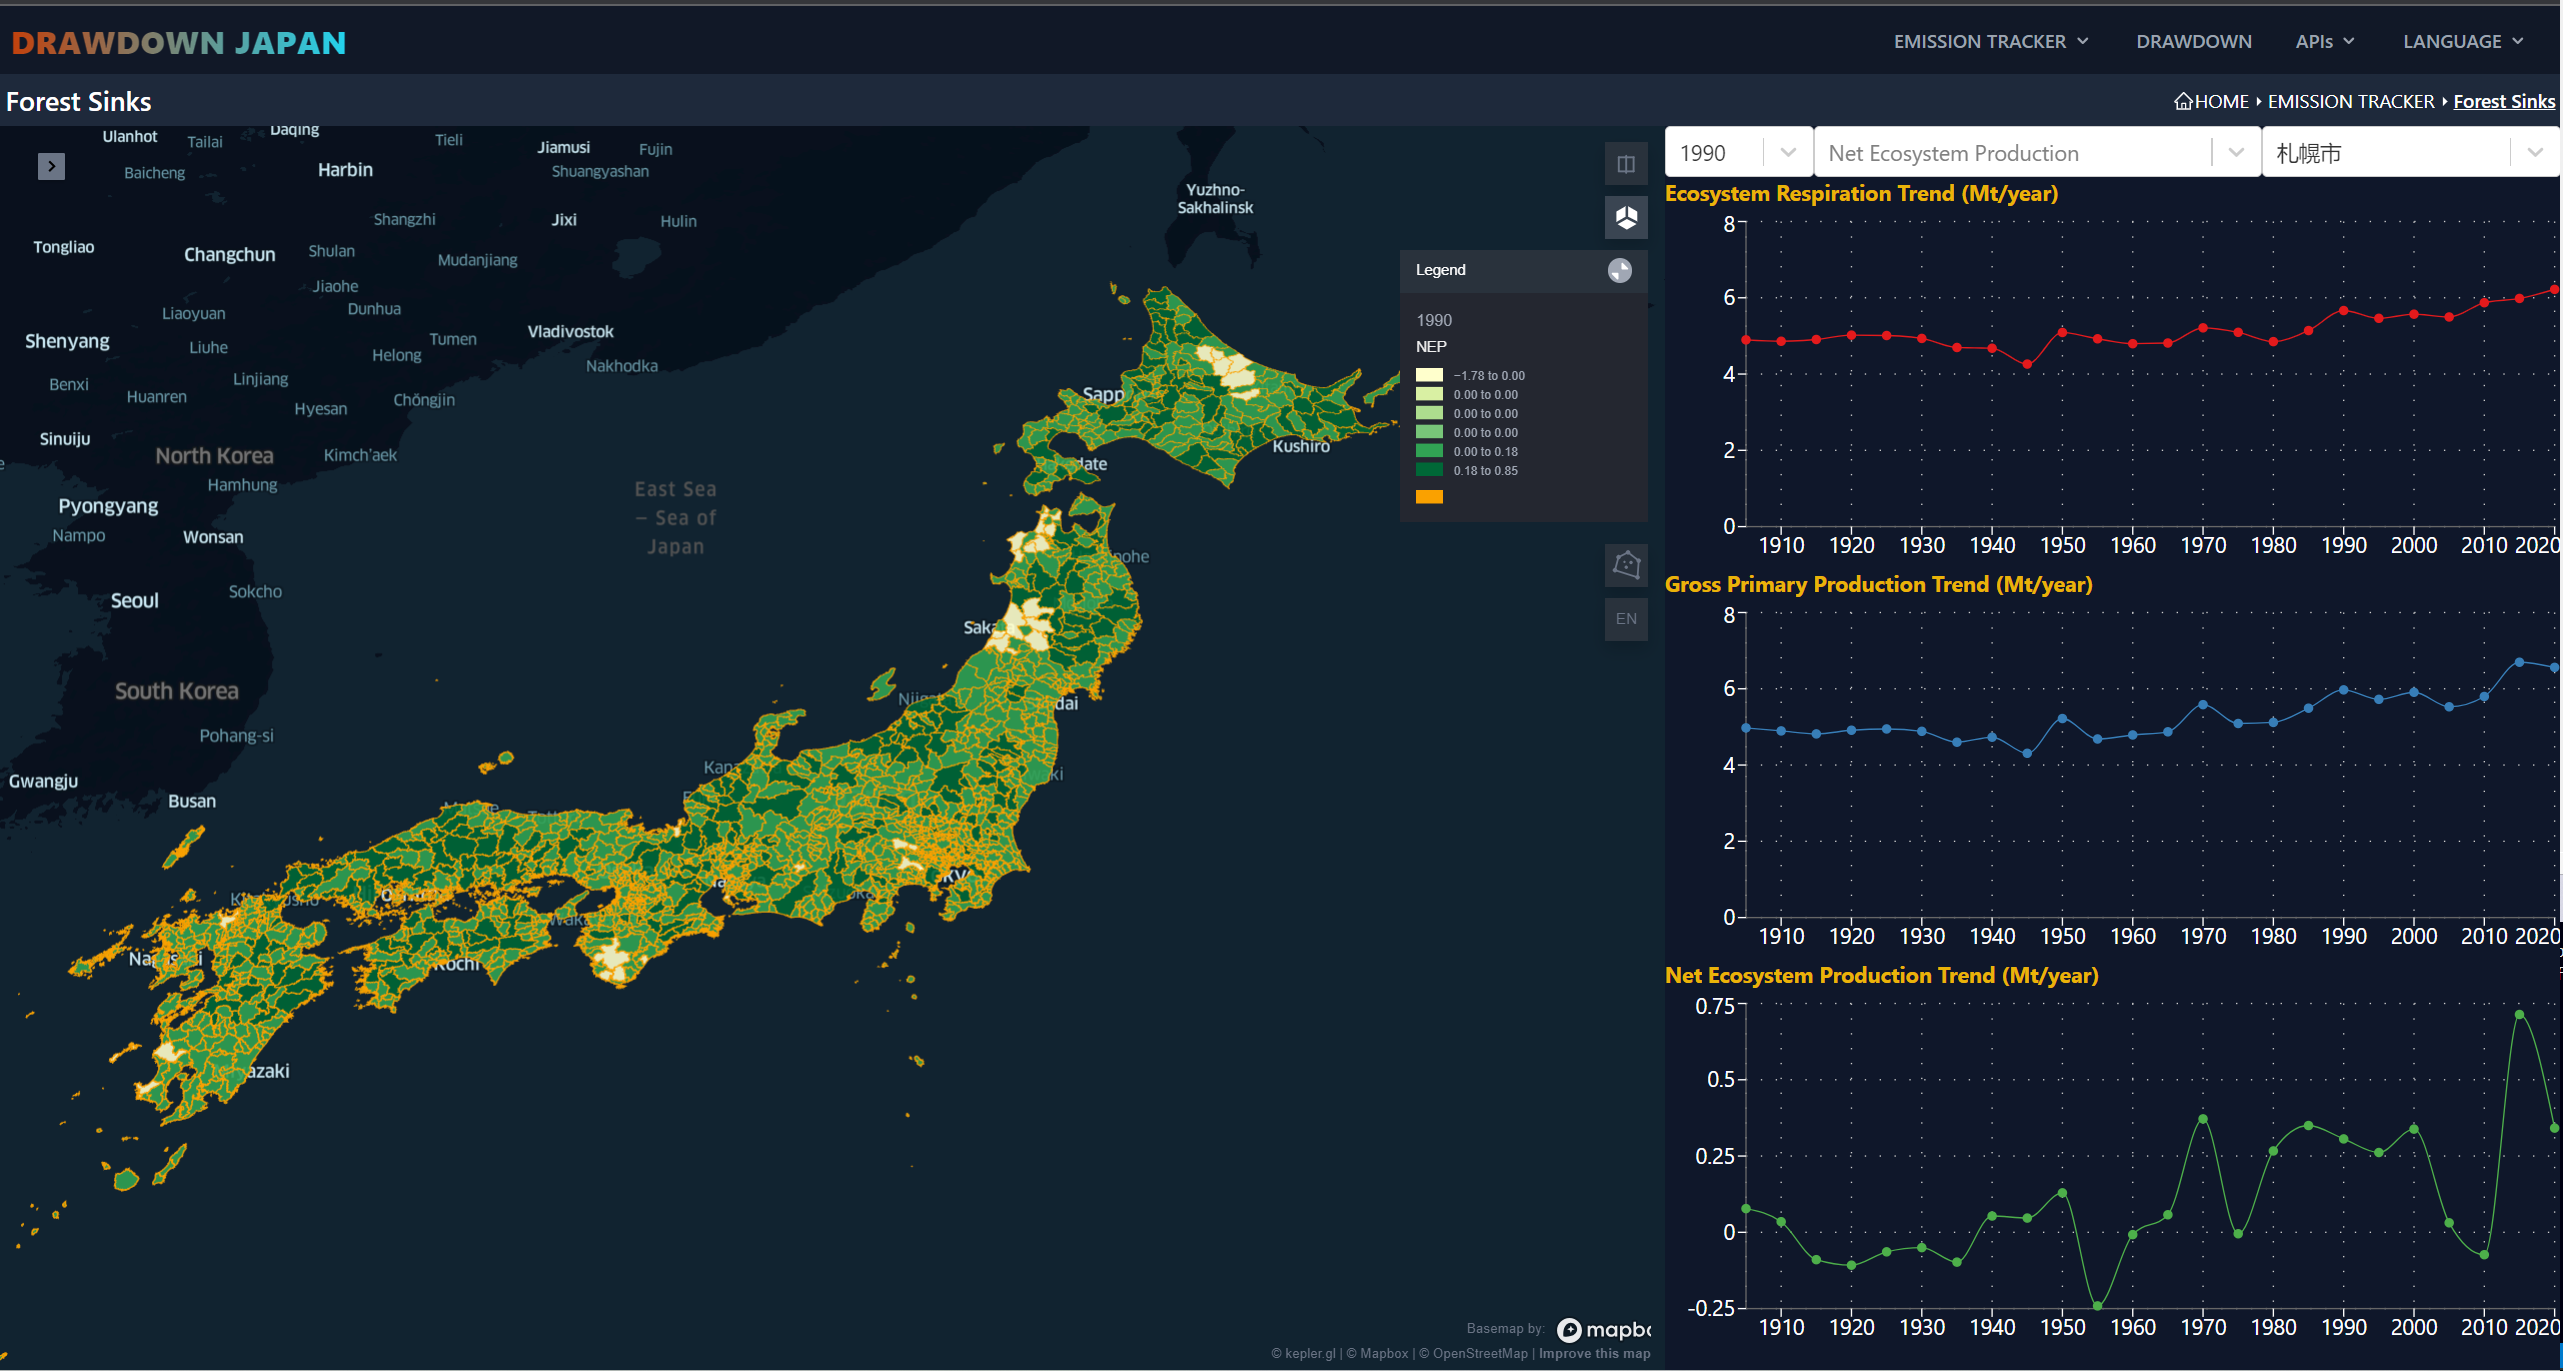
\includegraphics[width=.9\textwidth]{figs/chap7/ems_forest.png}
      \caption{Forest Sinks}
      \label{fig:chap7_fig_ems_tracker_d}
  \end{subfigure}%
  \begin{subfigure}{.5\textwidth}
      \centering
      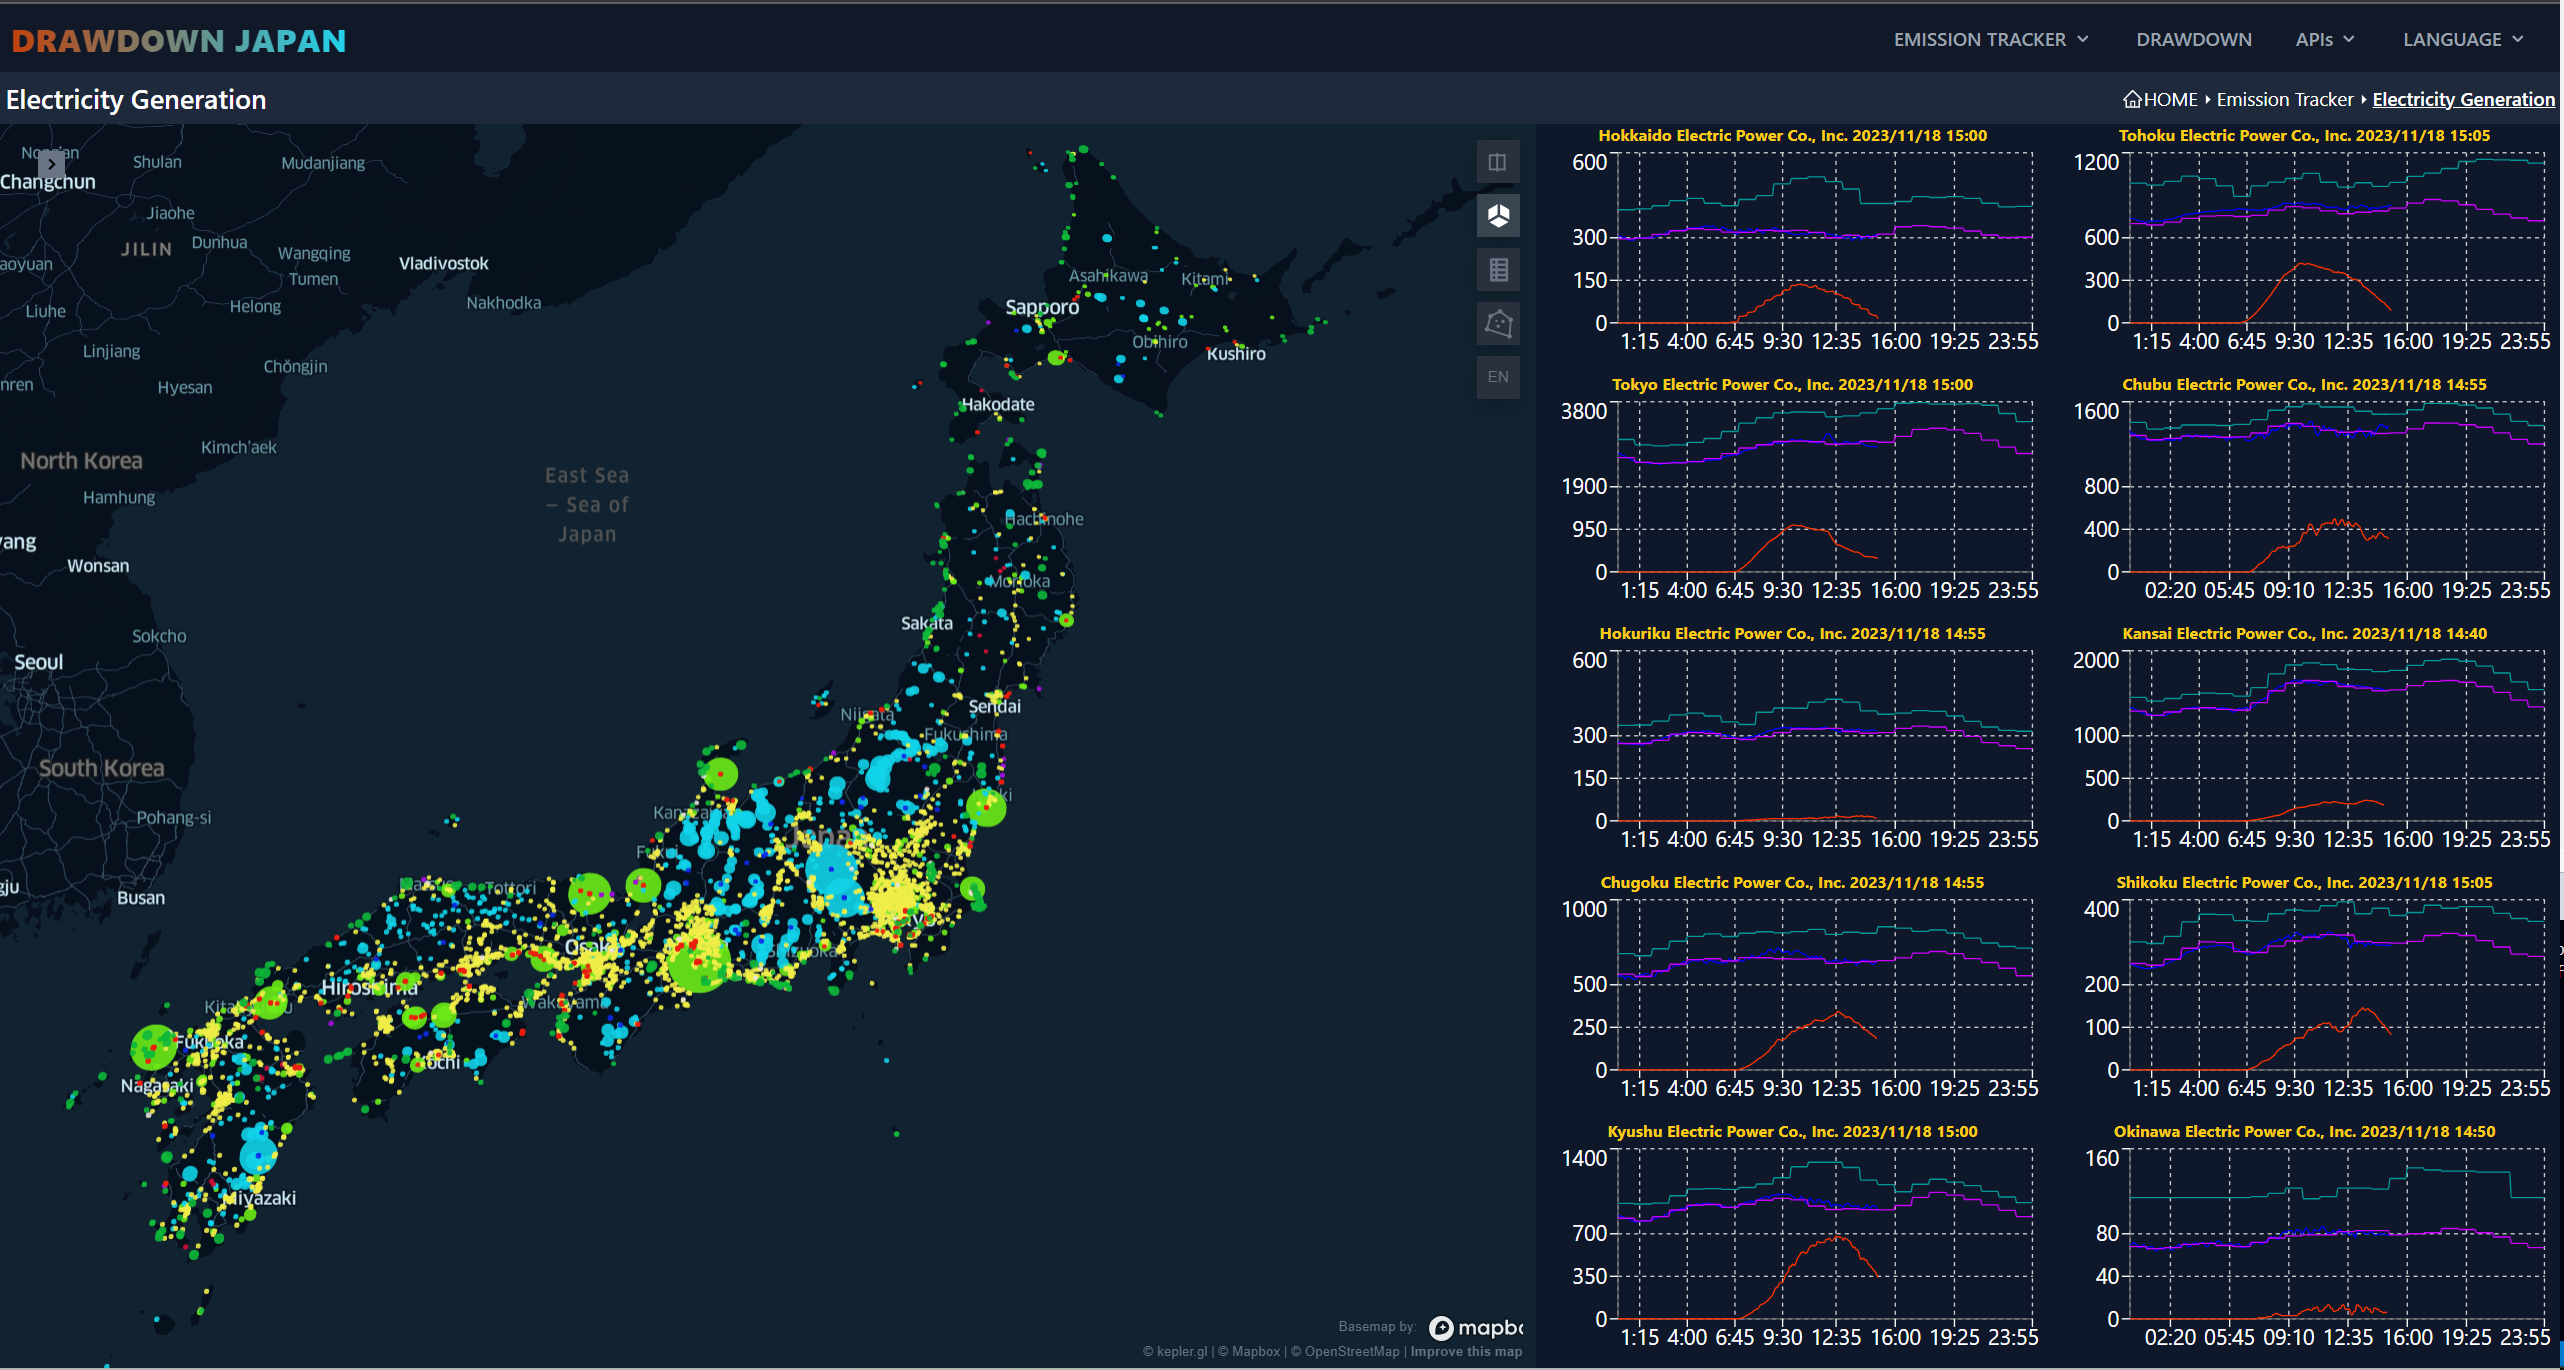
\includegraphics[width=.9\textwidth]{figs/chap7/ems_electric.png}
      \caption{Electricity Statistic}
      \label{fig:chap7_fig_ems_tracker_e}
  \end{subfigure}
  \caption{Emission Tracker interfaces}
  \label{fig:chap7_fig_ems_tracker}
\end{figure}

The Emission Tracker, depicted in Figure \ref{fig:chap7_fig_ems_tracker}, furnishes details about emissions and energy consumption at the municipal level. The visualized data is categorized into tabs, encompassing an overview of emissions, energy consumption, electricity statistics, industrial emissions, and forest sinks. Users can conveniently access pertinent information by choosing a municipality of interest through a dropdown selection box or a map.\par

[Emission Overview]: The content of this webpage, illustrated in Figure \ref{fig:chap7_fig_ems_tracker_a}, presents emission data categorized by sector (Industry, Consumer, Transportation, Waste) spanning from 1990 to 2019. This section offers insights into the current status and temporal fluctuations in emissions.\par

[Energy Consumption]: The contents of this webpage, depicted in Figure \ref{fig:chap7_fig_ems_tracker_b}, provide in-depth details regarding energy consumption at the municipal level in Japan spanning from 2013 to 2019. The data is compiled based on energy type and sector, aiding in decision-making processes related to efficient energy use and savings. \par

[Electricity Statistics]: The content on this webpage, illustrated in Figure \ref{fig:chap7_fig_ems_tracker_e}, presents details on the spatial distribution of power plants in Japan, categorized by plant type. The information encompasses data from major domestic power companies, covering electricity usage, usage forecasts, and supply forecasts. This data is sourced through the provided APIs from 10 major electric power companies, each representing a region in Japan (Table \ref{tab:chap7_tab1} contains the API endpoints for the data utilized in the platform, sourced from 10 electric companies). \par

[Industrial Emissions]: The content on this webpage, depicted in Figure \ref{fig:chap7_fig_ems_tracker_c}, provides a thorough perspective on industrial sector emissions. It displays emission profiles for each company (specific operators under the Energy Saving Act with a total energy usage of 1500kl/year or more) from 2009 to 2017. The webpage utilizes reporting information in accordance with the Energy Saving Act to consolidate municipal-level emissions, offering insights into the nationwide distribution of industrial emissions. Additionally, it ranks companies based on annual emissions within municipalities, serving as reference information for monitoring industrial sector emissions.\par

[Forest Sinks]: The content on this webpage, illustrated in Figure \ref{fig:chap7_fig_ems_tracker_d}, exhibits three crucial variables associated with forest absorption: Gross Primary Production (GPP), Net Ecosystem Production (NEP), and ecosystem respiration. These variables, obtained from simulations conducted by the global model Vegetation Integrative Simulator for Trace Gas (VISIT), depict a long-term trend spanning from 1901 to 2020. The data is presented at the municipal level, offering a rolling display of 5 years of data. \par
\begin{figure}[tbh!]
  \centering
  \begin{subfigure}{.5\textwidth}
      \centering
      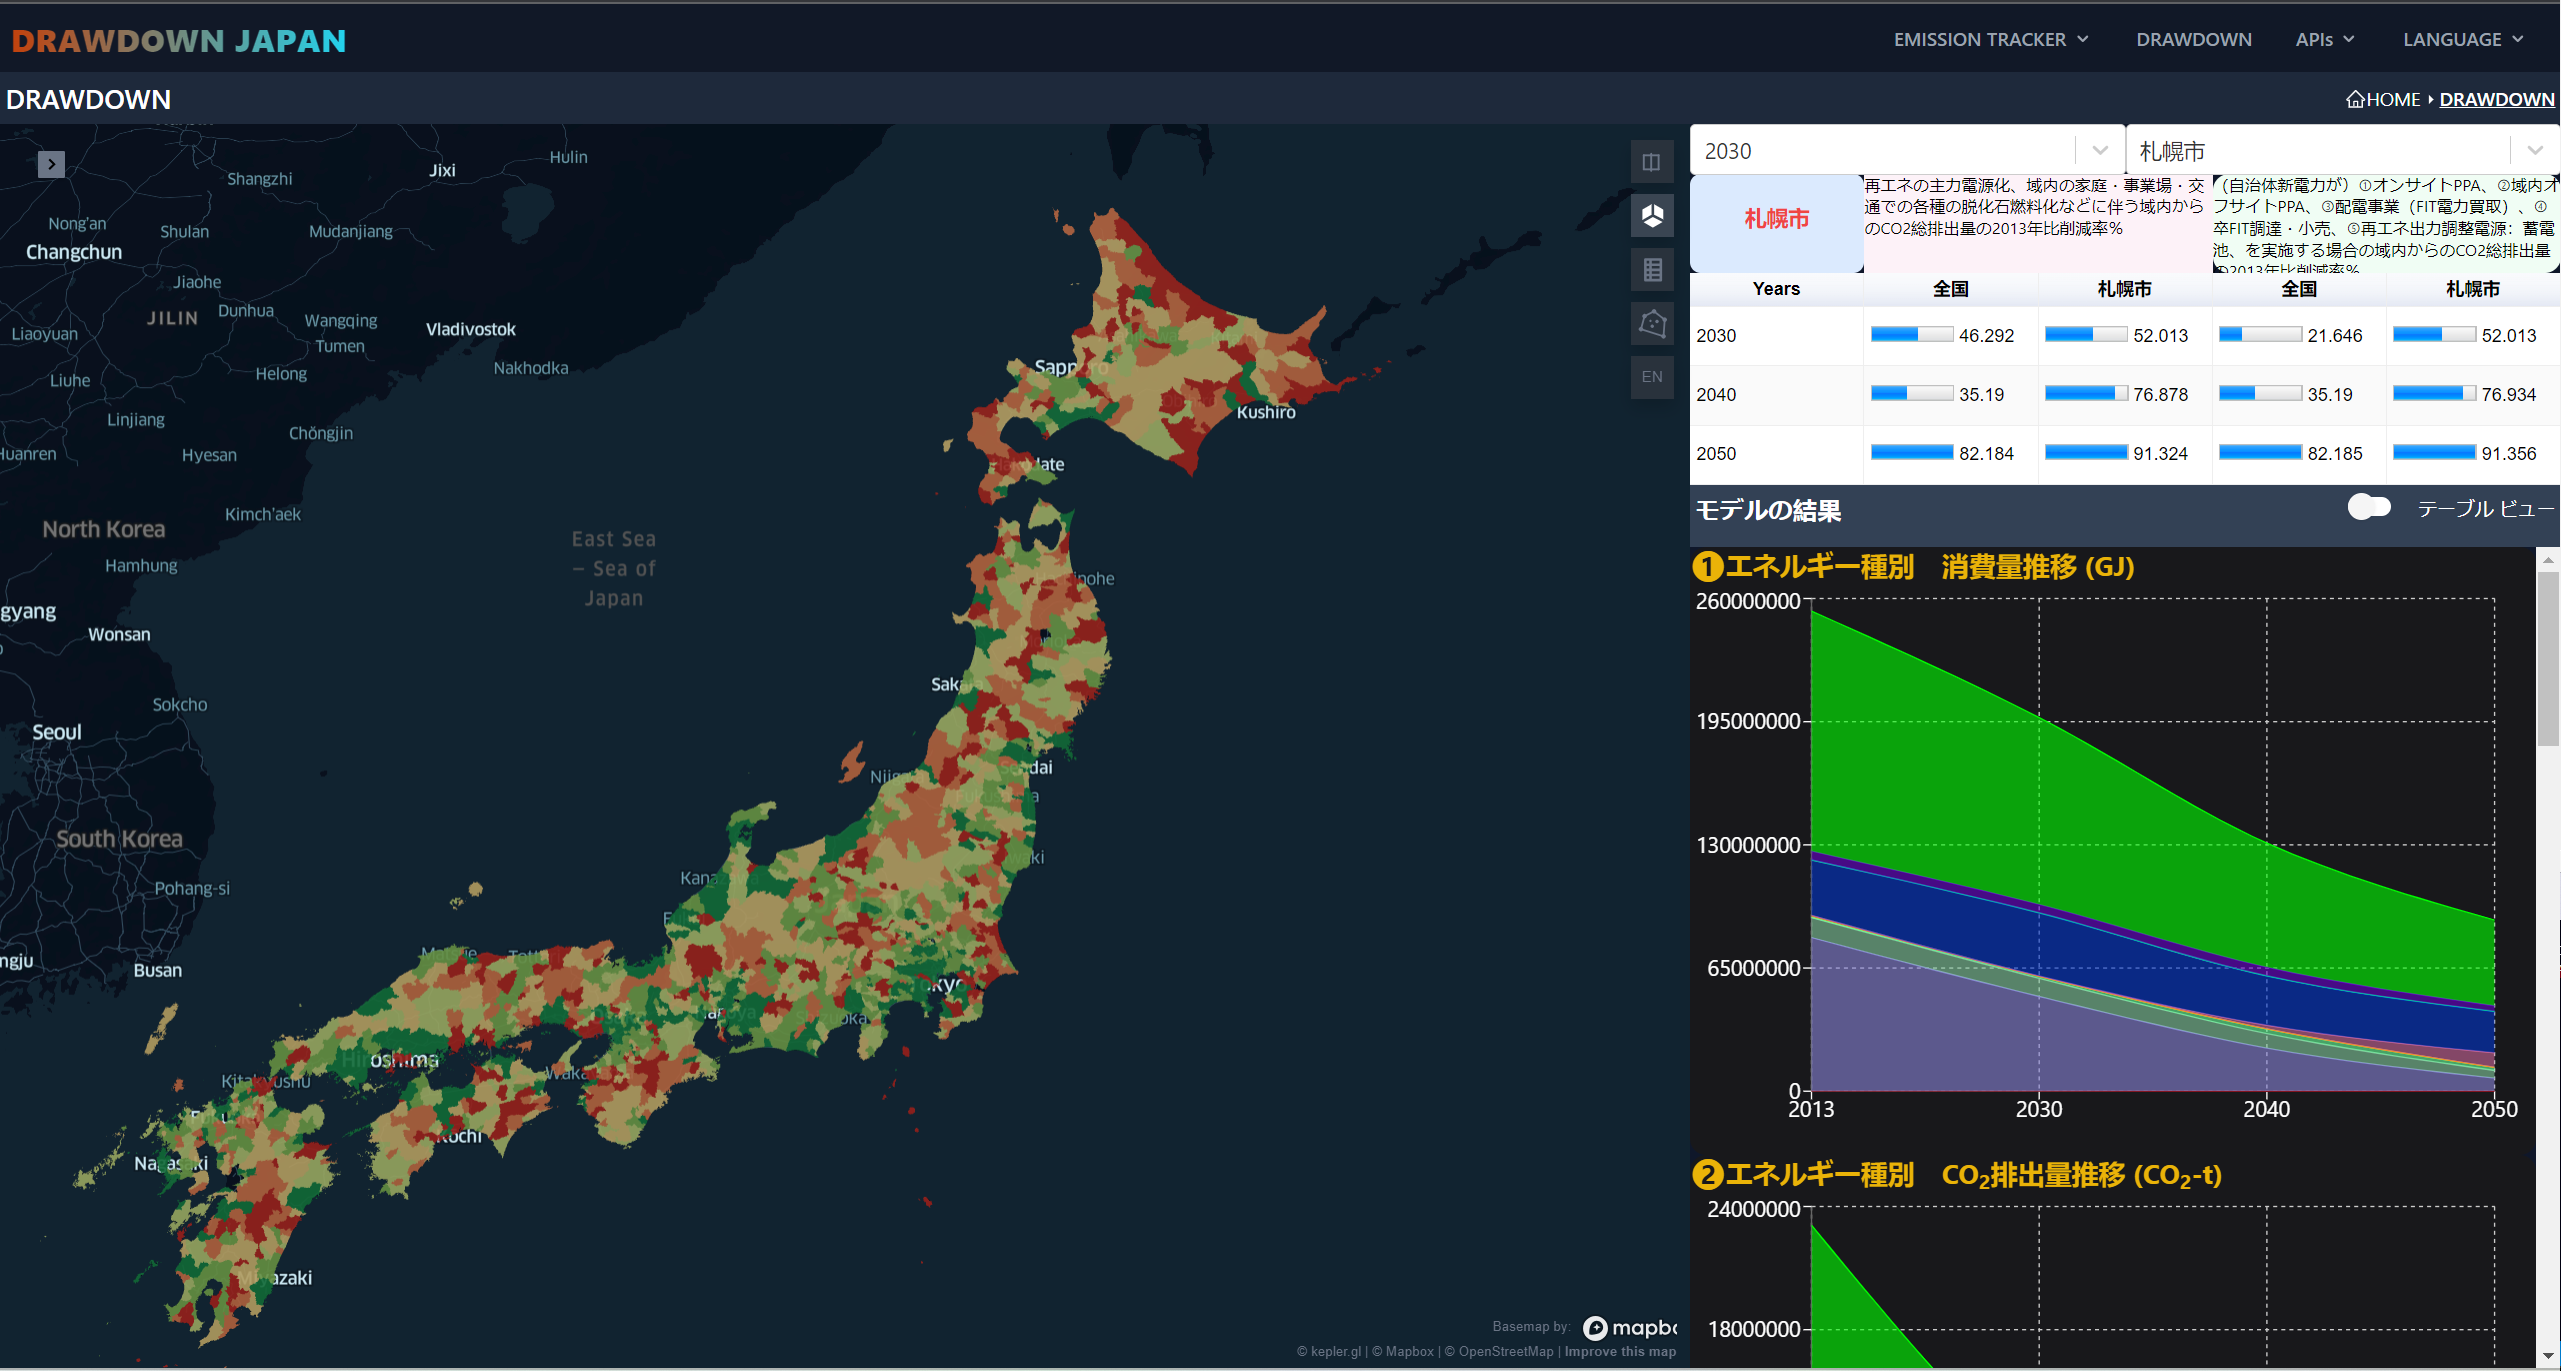
\includegraphics[width=.9\textwidth]{figs/chap7/drawdown1.png}
      \caption{Map and charts}
  \end{subfigure}%
  \begin{subfigure}{.5\textwidth}
      \centering
      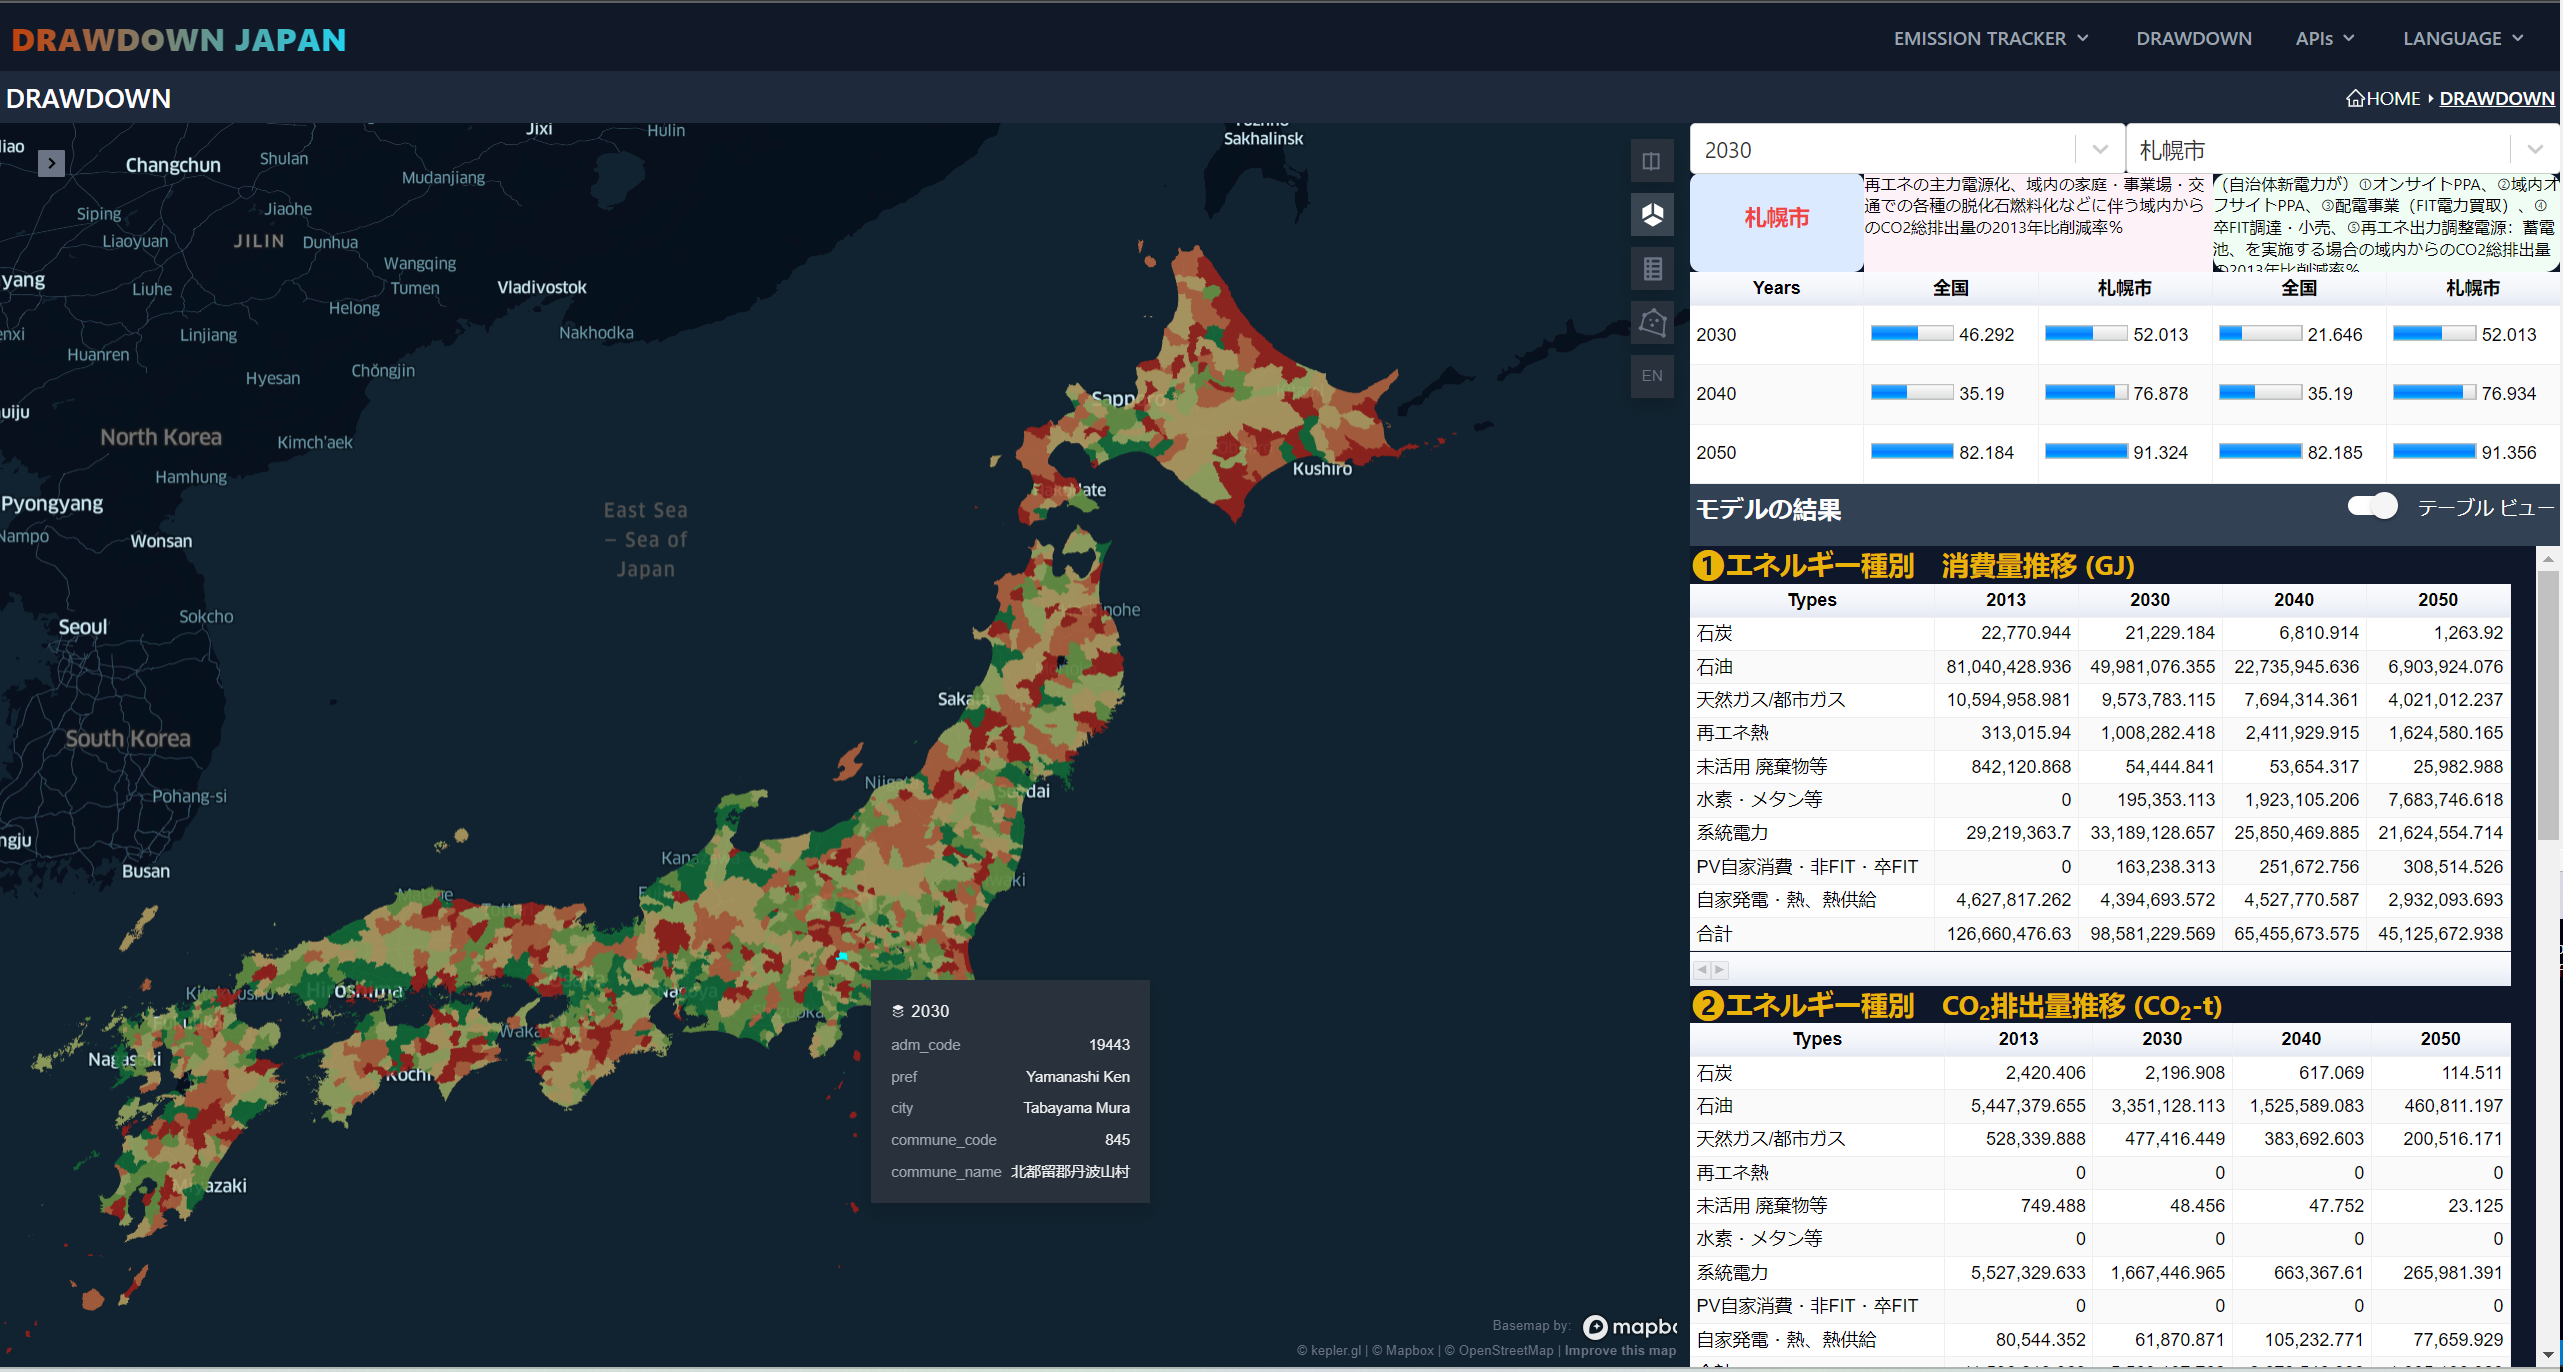
\includegraphics[width=.9\textwidth]{figs/chap7/drawdown2.png}
      \caption{Map and tables}
  \end{subfigure}
  \caption{Drawdown tab interfaces}
  \label{fig:chap7_fig_drawdown}
\end{figure}

The "Drawdown" page (refer to Figure \ref{fig:chap7_fig_drawdown}) outlines a comprehensive roadmap for achieving a reduction in CO\textsubscript{2} emissions by 2050 at the municipal level in Japan. Specifically, it provides a roadmap with diverse parameters, including trends in energy consumption, trends in CO\textsubscript{2} emissions by energy type, trends in CO\textsubscript{2} emissions by sector/industry, regional renewable energy electricity, regional production-consumption planning, and the ratio of total regional production-consumption to total energy usage. Additionally, it visually represents the total CO\textsubscript{2} emissions reduction by 2030, 2040, and 2050. This enables municipal officials not only to scrutinize their municipality's data intricately but also to enhance their understanding through personalized data comparisons with other similar municipalities. \par

\begin{figure}[tbh!]
  \centering
  \begin{subfigure}{.5\textwidth}
      \centering
      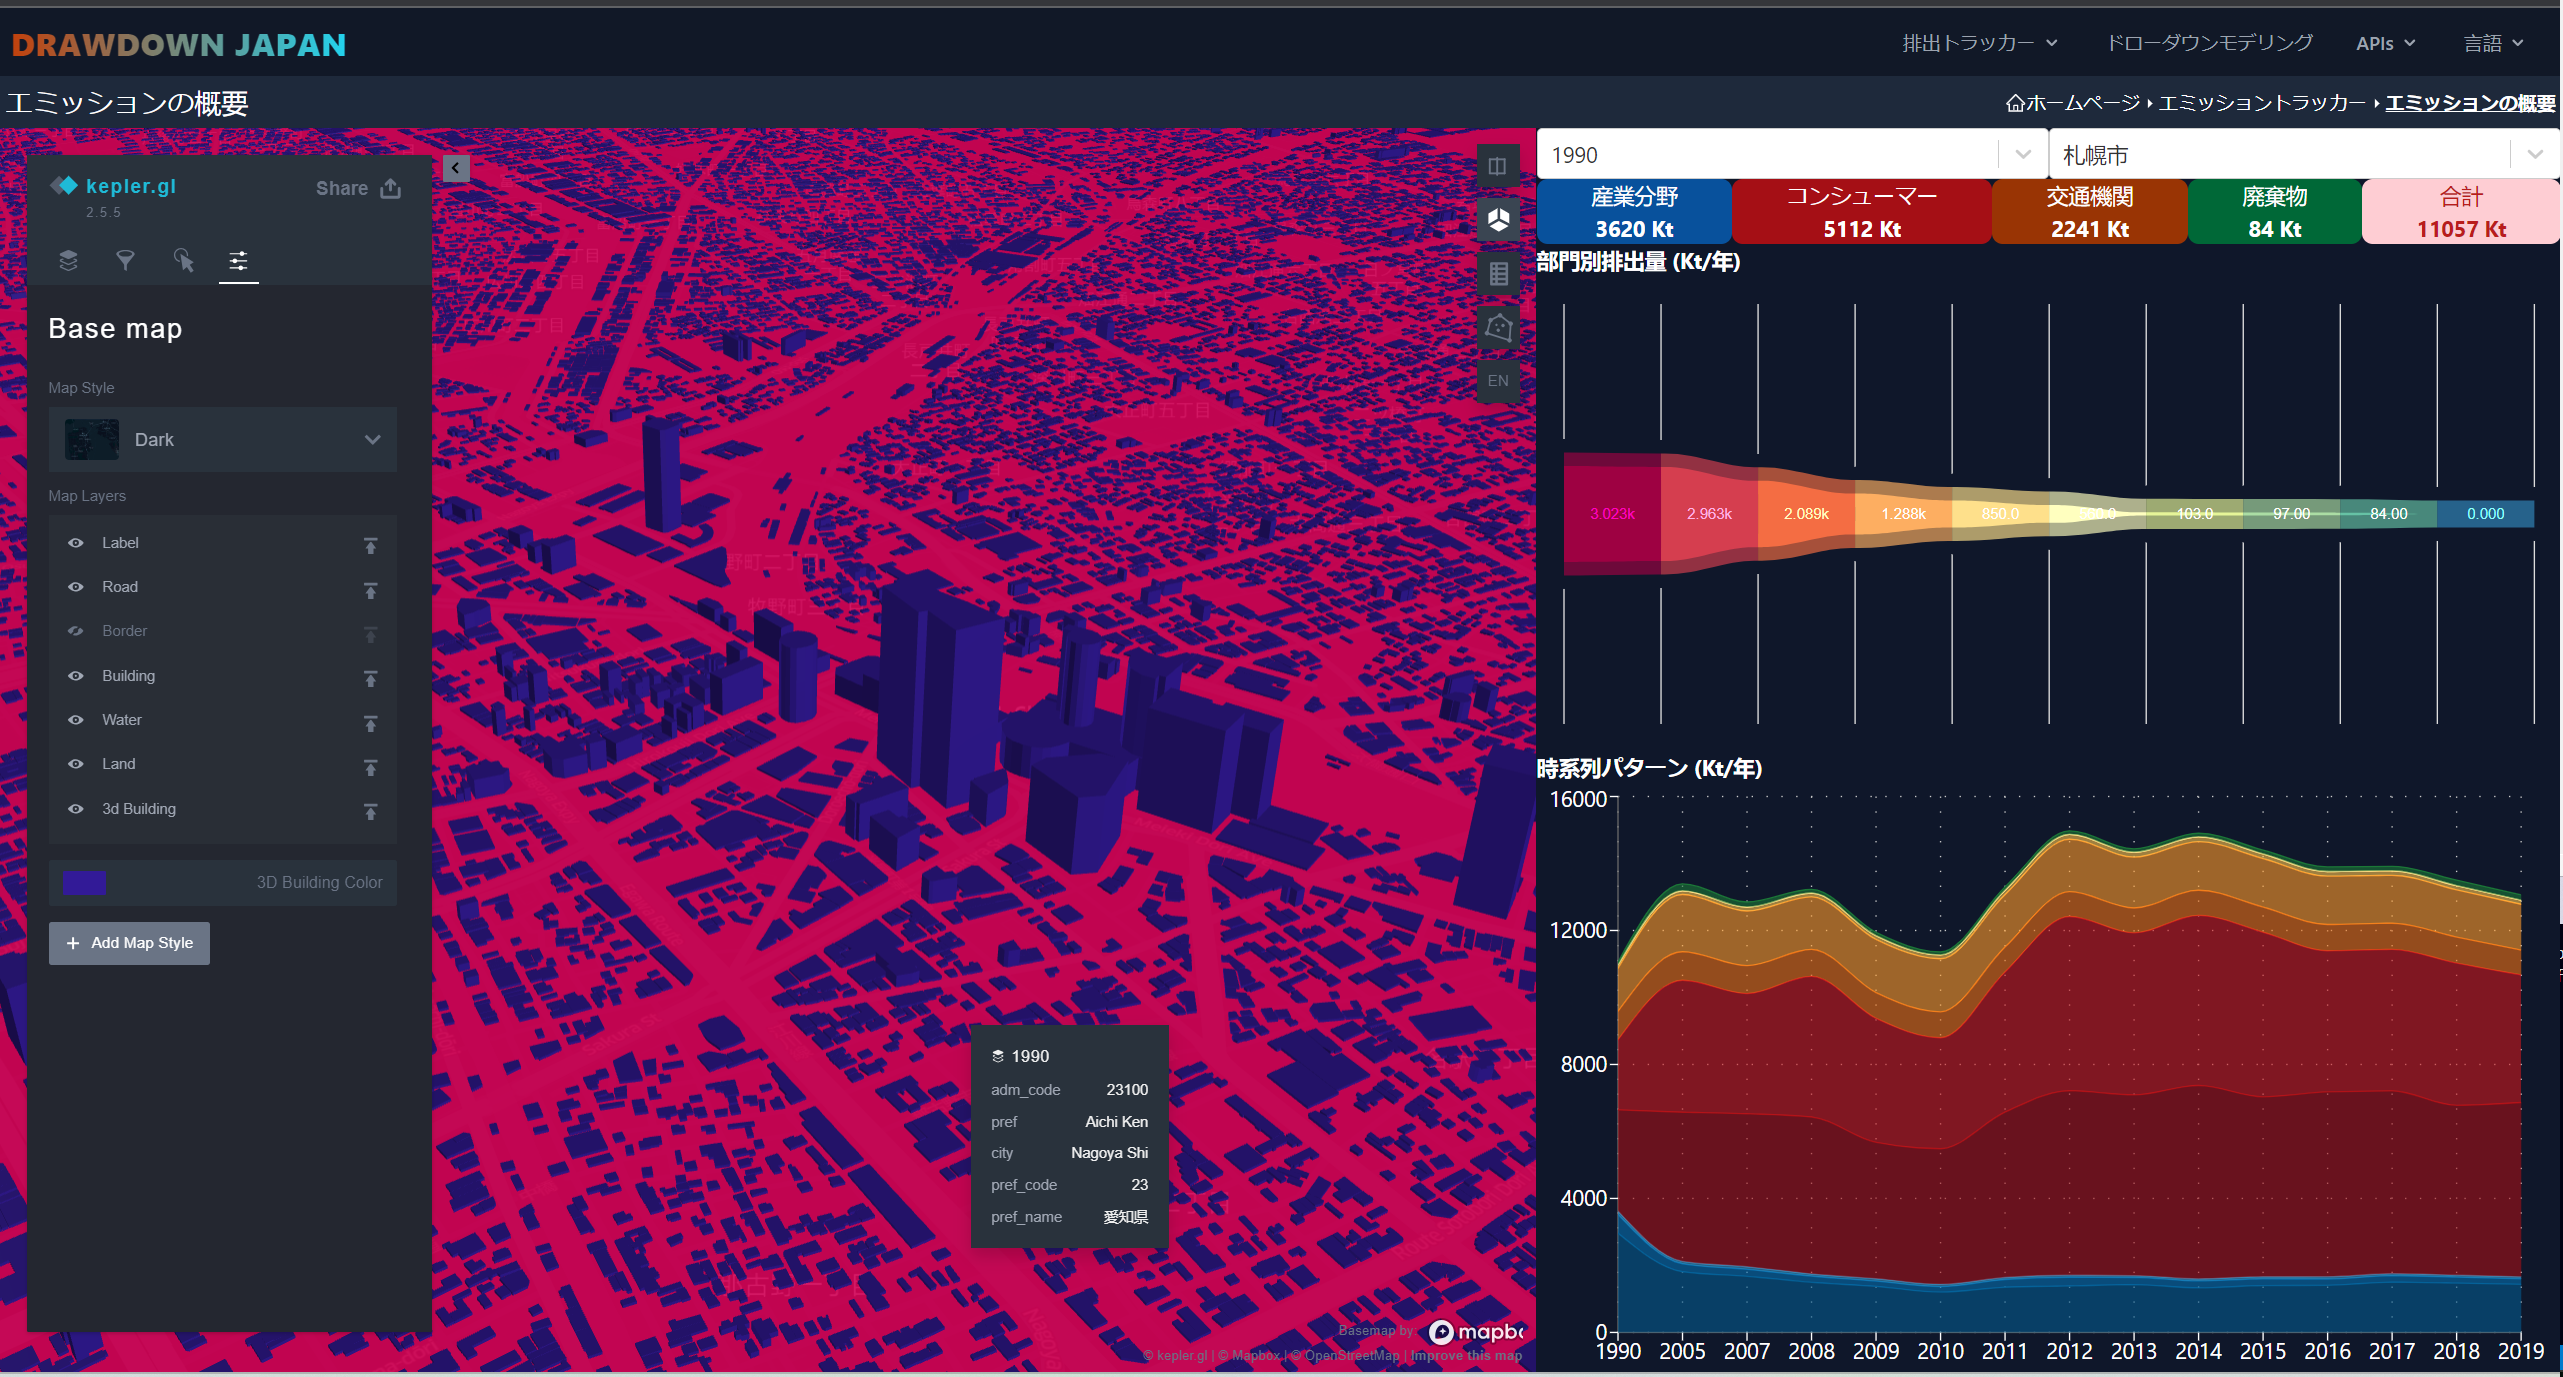
\includegraphics[width=.9\textwidth]{figs/chap7/3d_bldg.png}
      \caption{3D buildings visualization}
  \end{subfigure}%
  \begin{subfigure}{.5\textwidth}
      \centering
      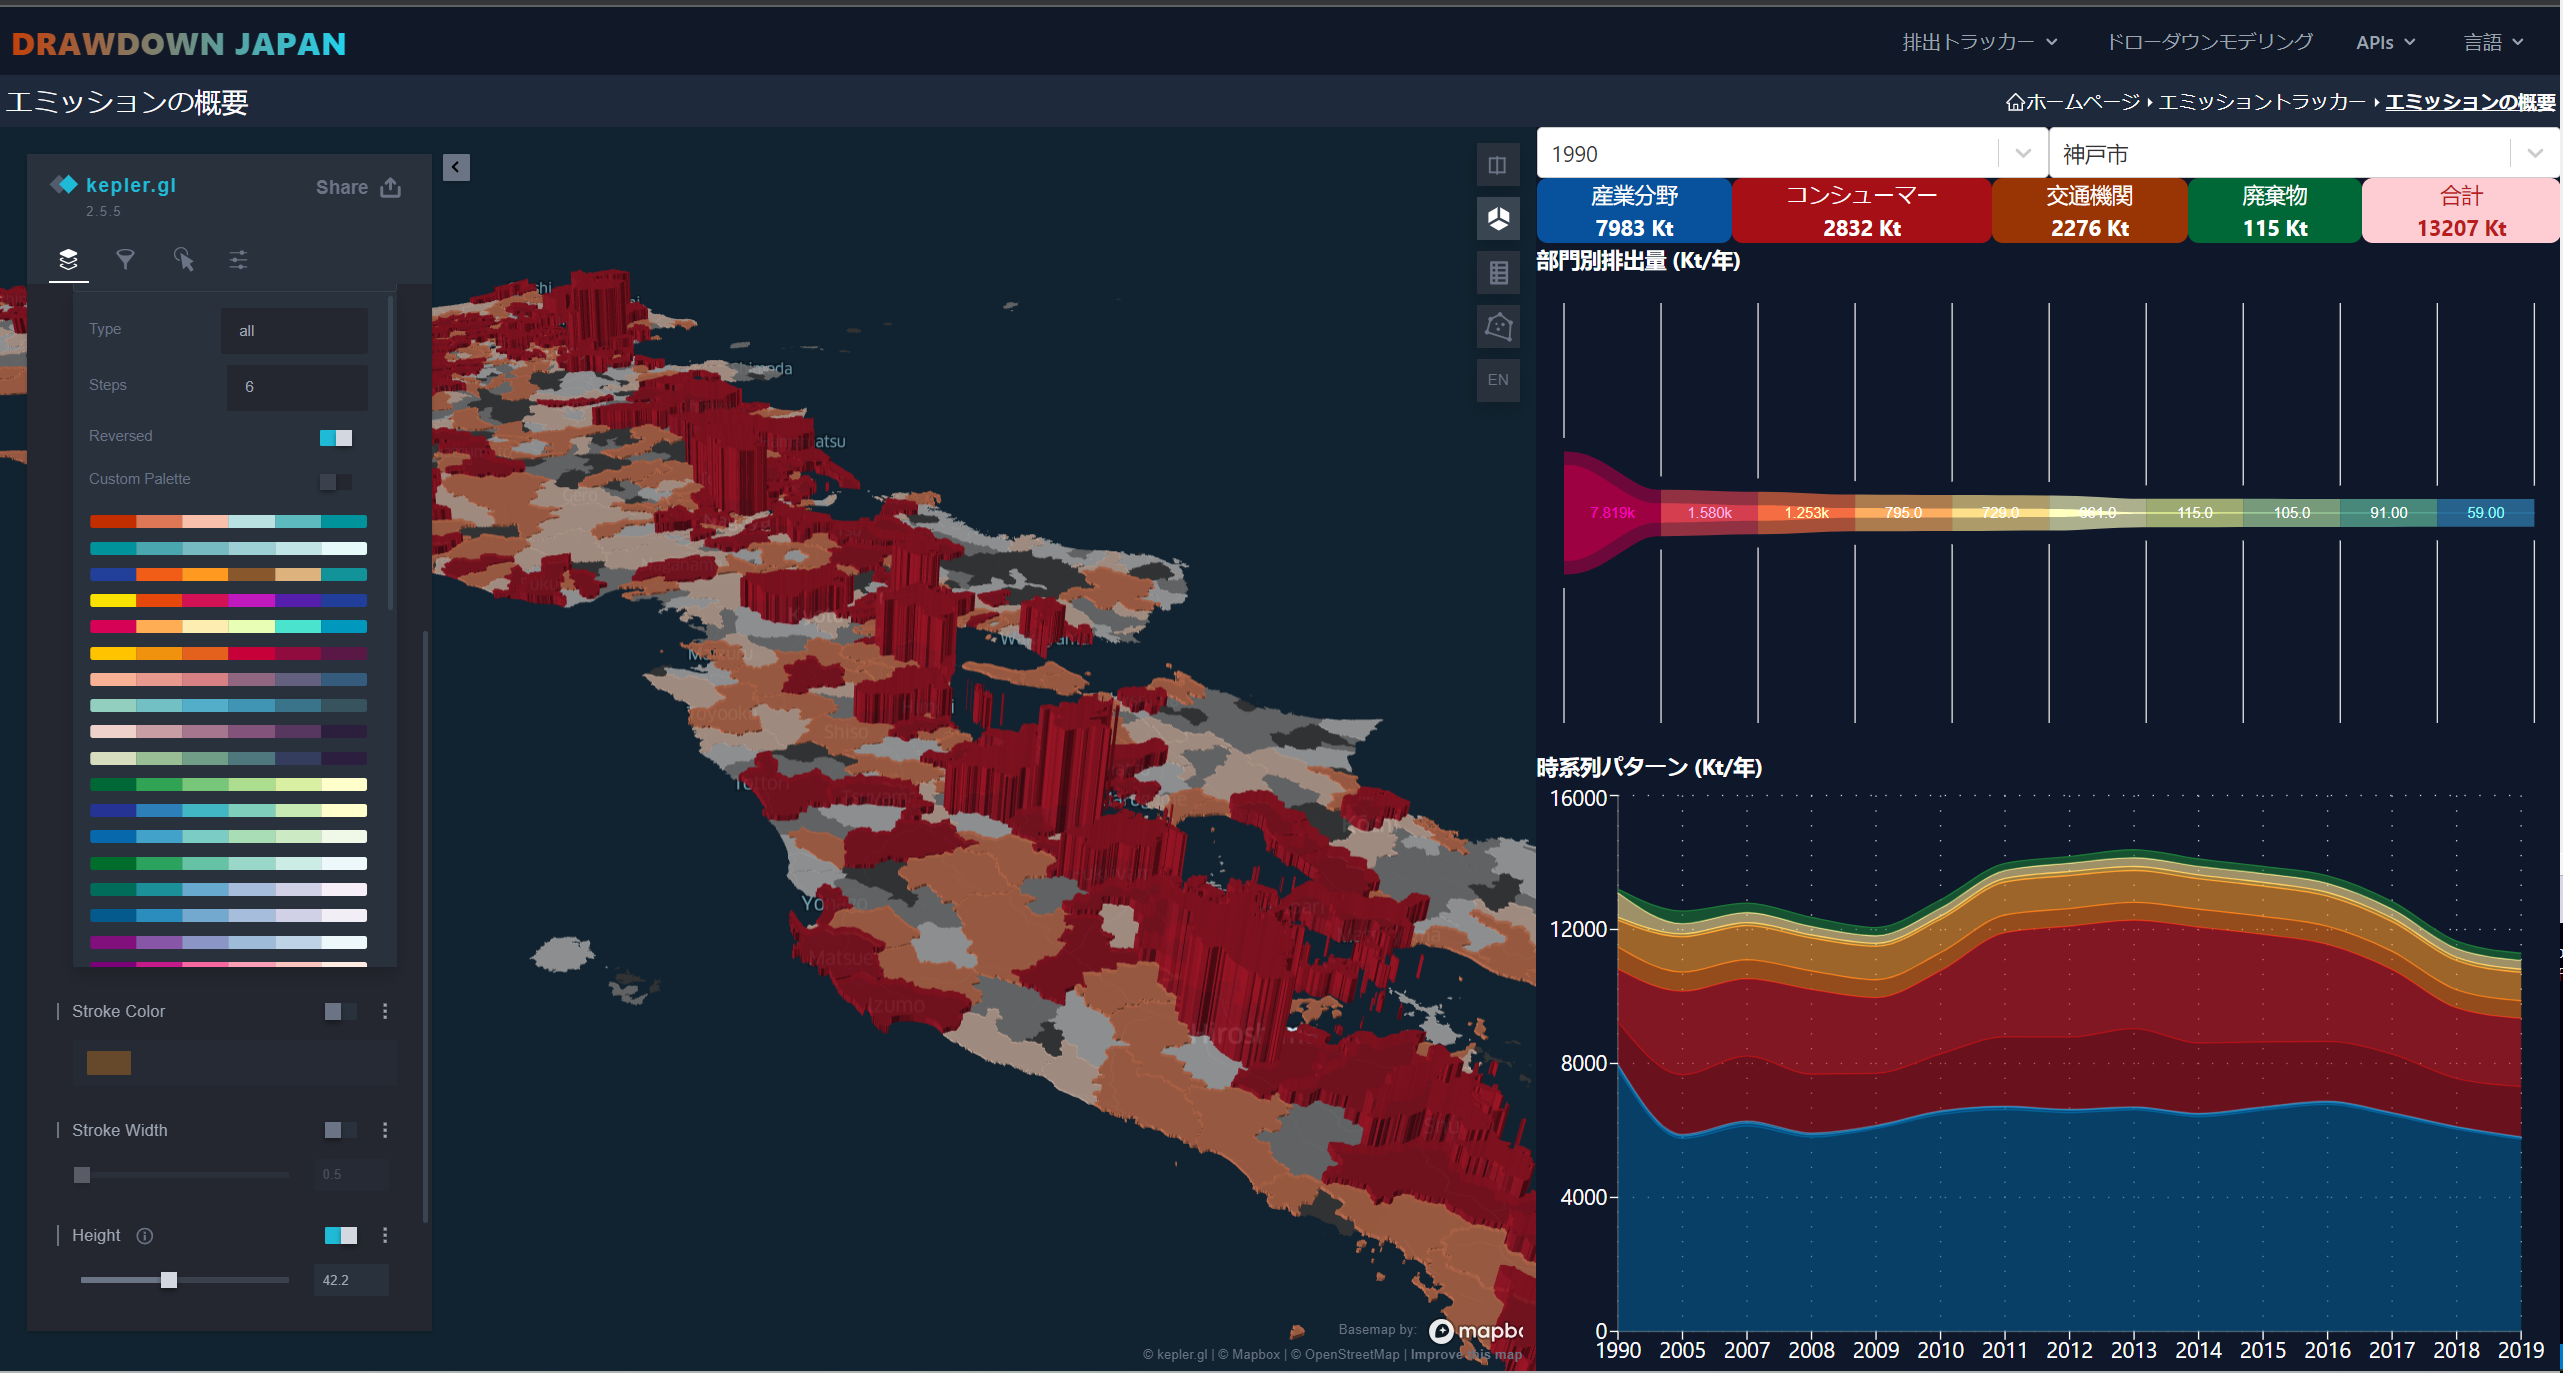
\includegraphics[width=.9\textwidth]{figs/chap7/3d_ja.png}
      \caption{Japanese text}
  \end{subfigure}
  \caption{Additional platform interfaces}
  \label{fig:chap7_fig_other_interface}
\end{figure}

In addition to the functionalities outlined earlier, as we incorporated Kepler.gl for map visualization, which enables end-users to customize the map personally with options such as 2D/3D views, color schemes, tooltips, and various settings (refer to Figure \ref{fig:chap7_fig_other_interface}). Users also have the capability to upload their own data for visualization and comparison with the provided data. Furthermore, we offer content in both English and Japanese to facilitate easy comprehension of information on our GIS platform. \par

The GIS platform is accessible at \url{http://de14.digitalasia.chubu.ac.jp/.}\par


\subsection{Discussion}

When comparing this GIS platform to existing platforms like Project Drawdown (refer to Figure \ref{fig:chap7_fig_other_gis_a}) and Drawdown Georgia \citep{brown2022carbon, brown2021translating} (refer to Figure \ref{fig:chap7_fig_other_gis_b}), the interface design may differ slightly, but the commonality lies in charts and maps being fundamental components.\par

\begin{figure}[tbh!]
  \centering
  \begin{subfigure}{\textwidth}
      \centering
      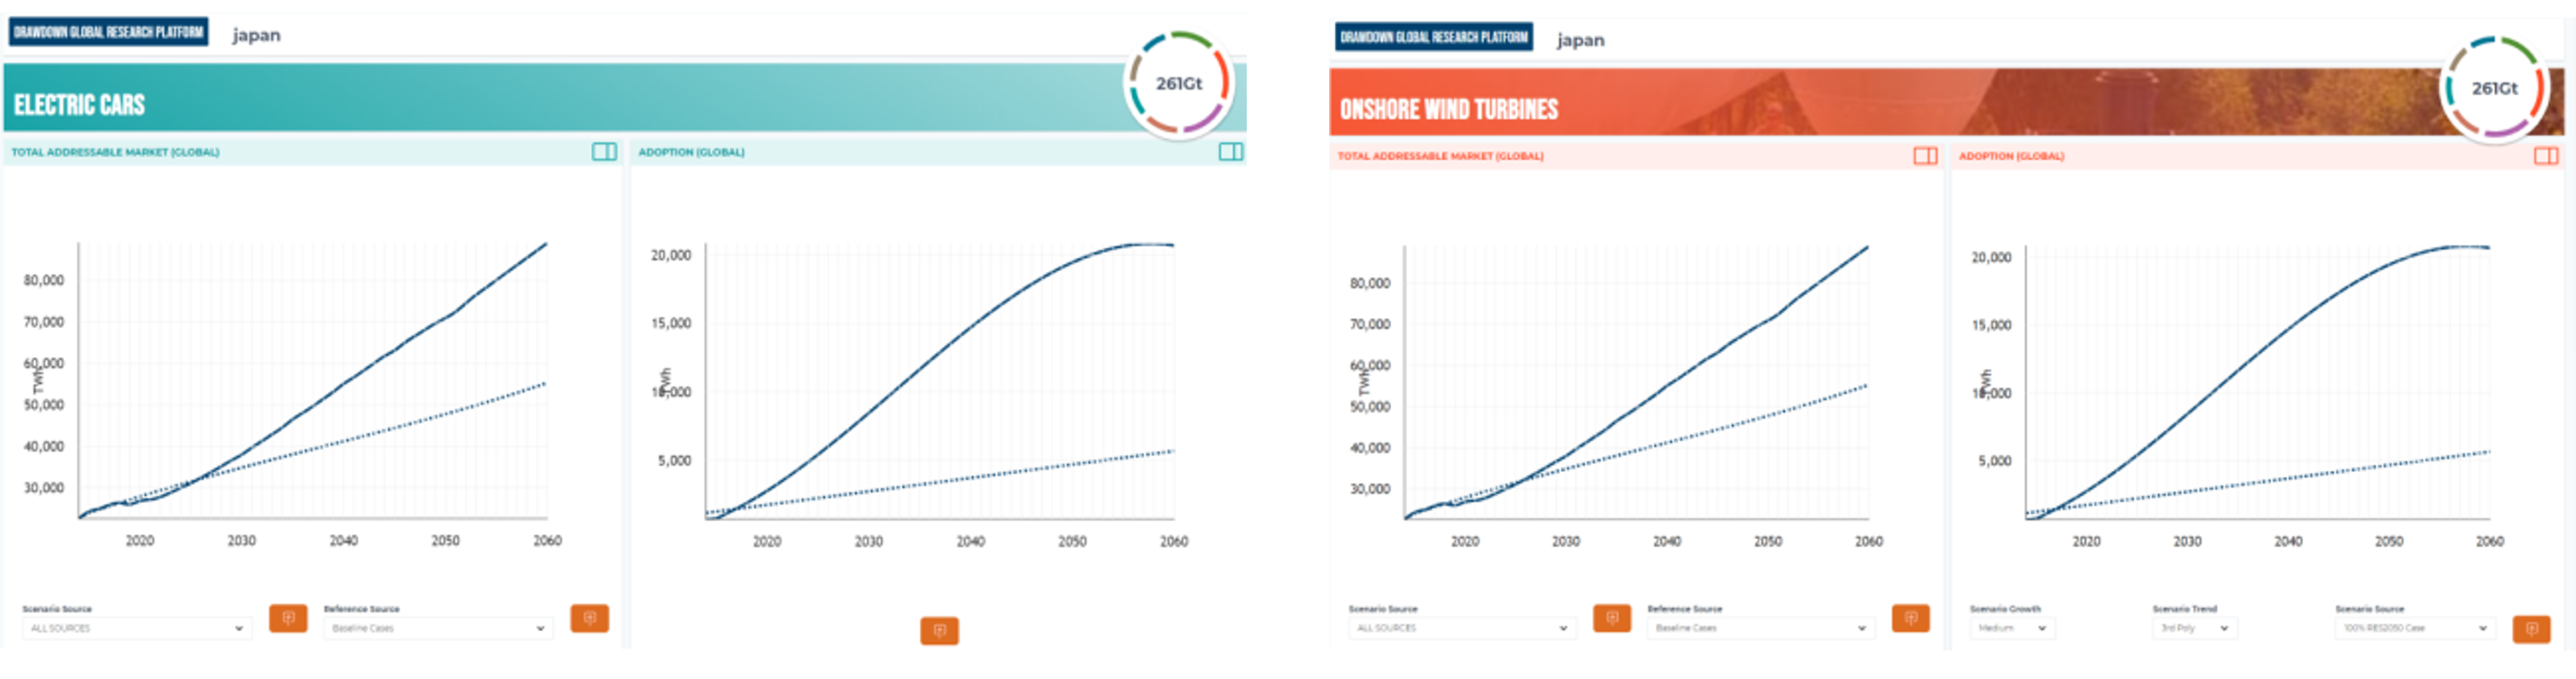
\includegraphics[width=.9\textwidth]{figs/chap7/project_drawdown.png}
      \caption{The Drawdown modelling interface of the Project Drawdown}
      \label{fig:chap7_fig_other_gis_a}
  \end{subfigure}

  \begin{subfigure}{\textwidth}
      \centering
      \includegraphics[width=.9\textwidth]{figs/chap7/drawdown_georgia.png}
      \caption{The GHG Tracker interface of the Drawdown Georgia project}
      \label{fig:chap7_fig_other_gis_b}
  \end{subfigure}
  \caption[Comparison with other platforms]{The interfaces of the Project Drawdown (a) and the GHG Tracker (Drawdown Georgia) (b)}
  \label{fig:chap7_fig_other_gis}
\end{figure}

The key distinction between this GIS platform and these existing platforms is that this platform has become an integrated Geo-portal, utilizing GIS for all components from emission tracking to drawdown modelling. This integration allows for a comprehensive representation of emission data and simultaneously provides a simulated roadmap, setting it apart from other platforms.\par
In the future, we plan to enhance the user interface based on user experience feedback and incorporate a global perspective into the system development.\par